\chapter{Calculus II: Indefinite Integration}
In Calculus I, we delved into the fundamental concepts of limits, derivatives, continuity, and tried to understand how things change. We learned how to find slopes of curves, calculate instantaneous rates of change, and understand the concept of a limit - and got somewhat comfortable with the idea that as we let things get infinitely close, we can figure out what's happening at a particular point. That was the beginning of our journey into understanding the mathematical underpinnings of change.\\
Now, as we move into Calculus II, we're going to take this journey a step further. We're going to explore the opposite process: instead of finding rates of change, we're going to learn how to work backward and find the cumulative effect of change over a range, and this is where integration comes into play. But why is this important?\\
Well, calculus isn't just an abstract exercise in mathematical manipulation. It's the language of the universe. From understanding how objects move under the influence of forces to predicting the spread of diseases in a population, calculus is the tool we use to describe and make sense of the real world. Think of it as both a powerful microscope and telescope that allows us to zoom in and out on nature's processes.\\
Integration helps us calculate areas, accumulate quantities, and understand the net effect of change over time. Whether you're an engineer designing a bridge, a physicist modeling the motion of planets, an economist analyzing markets, or a biologist studying population growth, you'll find integration to be a fundamental tool.\\
So, let's get started on this adventure together. Calculus II is where we dig deeper into the mathematical tools that shape our understanding of the universe. It's going to be exciting, challenging, and, I hope, a lot of fun. Welcome to the world of Calculus II!\\
\section{The Fundamental nature of graphs}
We begin this chapter with a theorem which while of no practical use, is of great impotence to the foundations of Calculus.\\
\begin{theorem}
[Extreme value theorem]
    For a function $f(x)$ continuous between $[c,d]$ attains some maximum value $f(a)=M$ such that $f(a)=M\geq f(X)$ for all $x,a \in [c,d]$\\
    We also claim that a $f(b)=m$ exists such that $f(b)=m\leq f(X)$ for all $x,b \in [c,d]$ using the fact that $-f(x)$ is also continuous and it's maxima also exists.
    \begin{figure}[ht]
        \centering
        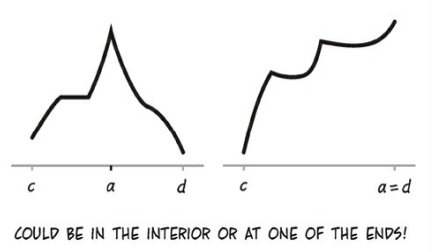
\includegraphics[width=0.5\linewidth]{Photos/Extreme value theorem.png}
        \caption{Extreme Value Theorem}
        
    \end{figure}
\end{theorem}
I have not included the complete rigorous proof of this. However, I'll try to give you an intuitive understanding of the same.\\
Let's assume that our theorem is false, that we don't have $f(a)=M \geq f(x)$ for $x,a \in [c,d]$. This means that for some values of $x \in [c,d], f(x)=\pm \infty$. Let one of those points be $g$. Therefore we can say, $\lim_{x \to g}f(a)$ is infinite limit at $x=g$ making all its neighbours(an infinite of them) incomparable to each other. However, if we have an infinite limit, which we know is not continuous, this will violate the assumption that $f(x)$ is continuous. Hence, our assumption is false and we there exists a $f(a)=M \geq f(x)$ for $x,a \in [c,d]$.\\
Using the extreme value theorem we can get:\\
\begin{theorem}
    [Rolle's Theorem]
    If $f(x)$ is continuous in $[c,d]$ and differentiable in $(c,d)$, and $f(c)=f(d)=0$, then there is atleast one point $a \in (c,d)$ such that $f'(a)=0$\\
\end{theorem}
While all this may sound like strange jargon, but it basically says that between any two roots of $f(x)$ we have one point of maxima, minima or inflection. While it is intuitively correct, as we did in Calculus I, here is the more formal version:\\
\begin{proof}
    If $f$ is the constant function $f(x) = 0$, then the result is obvious.\\
    If $f$ is not constant, then it has non-zero values. Therefore, it attains either a maximum $M > 0$ or a minimum $m < 0$ at some point $a$, by the Extreme Value Theorem. As $a$ is not one of the endpoints because $M,m \neq 0$, and hence, $f'(a)=0$\\
\end{proof}
And this finally gives rise to another theorem:\\
\begin{theorem}
    [Mean Value Theorem]
    If $f(x)$ is continuous in $[c,d]$ and differentiable in $(c,d)$, then there is a point $a \in (c,d)$ such that $f'(a)=\frac{f(d)-f(c)}{d-c}$\\
\end{theorem}
\begin{proof}
    Let's define a new function by changing the axis of $f(x)$ by making the chord from $c$ to $d$ the y axis. This can be done simply by subtracting  the chord from the function.\\
    $g(x)=f(x)-\frac{f(d)-f(c)}{d-c}(x-c)-f(c)$
    Then using Rolle's theorem we can claim that there exists $g'(a)=0$ where $a \in [c,d]$\\
    as $g'(x)=f'(x)-\frac{f(d)-f(c)}{d-c}\\
    \therefore g'(a)=f'(a)-\frac{f(d)-f(c)}{d-c}\\
    \iff 0=f'(a)-\frac{f(d)-f(c)}{d-c}\\
    \iff f'(a)=\frac{f(d)-f(c)}{d-c}$\\
    Hence, proved.
\end{proof}
You should notice that these theorems just say that a point fulfilling some conditions exist. They don't find such points or reveal anything about their nature.\\
Such theorems are called non-constructive.\\
\section{Integration}
Let's again think about our car example. If we know the speed of the car and the time it travelled at that speed we can easily find it's distance by simply multiplying the numbers.\\
What if we knew its speed in the first interval and then its speed in second interval and so on? You would say that the distance traveled is the multiplication of the velocity by the length of the interval. More mathematically, you would say it is $\sum_{i=1}v_it_i$ where the sequence $v_1,v_2, \dots$ is the collection of speeds in the intervals $t_1,t_2,\dots$.\\
\begin{figure}[ht]
    \centering
    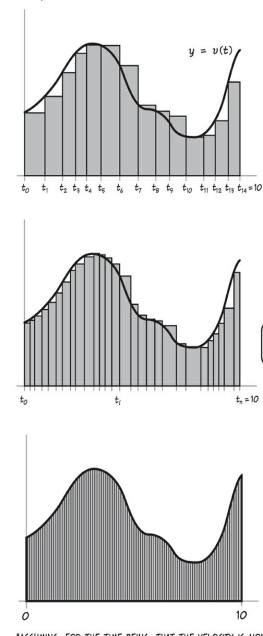
\includegraphics[width=0.5\linewidth]{Photos/The integral.png}
    \caption{The Integral}
\end{figure}
What if the velocity function had some closed form as a function $f(t)$ of time? Then one particular speed would only be for an infinitely small interval which we can write in Leibniz notation as $dt$. Hence, the distance traveled can be written as $\sum f(t) dt$. However, $\sum$ is used when we put integer values, but time is continuous and we need all real values between the integers.\\
We write this using a new notation known as the integral.\\
$\int^{t_{\text{final}}}_{t_{\text{initial}}} f(t) dt$
Here, you may wonder that as addition is easier then division, why did we not do integral first and then derivatives?\\
Let's try to solve the integral. We can through the picture attached notice that the integral is just the area under the graph. If I consider a small interval $h$ and consider that the area under the graph changes as our range of integration change(which is obvious), by some function $A(x)$ which is also continuous if $f(x)$ is continuous.\\
We can say that:
$A(t+h)-A(t)=f(t) \cdot h$ as $h \to 0$\\
$\therefore f(t)=\frac{A(t+h)-A(t)}{h}, h \to 0$ which is the definition of differentiation.\\
$\therefore f(t)=A'(t) \iff f'(t)=A(t) \iff f'(t)=\int f(t)dt$\\
This relates integration with differentiation which gives us the fundamental theorem of calculus(not the fundamental equation, that was the mouse-flea theorem)\\
\begin{theorem}
    [Fundamental Theorem of Calculus]
    $\int f'(x) dx = f(x)$
\end{theorem}
However, integration tends to be a bit tougher(an understatement)\\
\section{Techniques of indefinite Integration: Substitution}
When we don't put limits on the integration and are only interested in the function describing the area $A(x)$ we call it an indefinite integration. We generally find the anti derivative and add a constant $C$ to it.\\
A lot of people planning to give MCQ exams skip it as it is tricky and then just differentiate the four/five options. Examiners therefore nowadays put in some random values as the limits of the integration to force the candidate to compute the exact integral.\\
However, all of this is not as difficult if we are clear with Calc I.\\
\begin{theorem}
\begin{enumerate}
    \item $\int x^n dx = \frac{x^{n+1}}{n+1} + C$\\
    \item $\int \frac{1}{x} dx = \frac{-1}{x}+C$\\
    \item $\int \frac{1}{\sqrt{x}} dx = 2\sqrt{x}+C$
    \item $\int \frac{1}{x} dx=\ln{x}+C$\\
    \item $\int e^x dx = e^x+C$\\
    \item $\int a^x dx = \frac{a^x}{\ln{a}}$
    \item $\int \sin(x) dx = -\cos(x) + C$
    \item $\int \cos(x) dx = \sin(x) + C$
    \item $\int \sec^2(x) dx = \tan(x) + C$
    \item $\int \csc^2(x) dx = -\cot(x) + C$
    \item $\int \sec(x)\tan(x) dx = \sec(x) + C$
    \item $\int \csc(x)\cot(x) dx = -\csc(x) + C$
    \item $\int \frac{1}{\sqrt{1-x^2}}dx=\arcsin(x)+C$
    \item $\int \frac{1}{1+x^2}dx=\arctan(x)+C$
    \item $\int \frac{1}{x\sqrt{x^2-1}}dx=\sec^{-1}(x)+C$
\end{enumerate}
\end{theorem}
This all seems like a revision of Calc-I doesn't it?\\
Let's now look at some real integrals\\
\begin{theorem}
    \begin{enumerate}
        \item $\int \tan(x) dx = -\ln{|\cos(x)|} +C = \ln{\sec(x)}+C$
        \item $\int \cot(x) dx = \ln{|\sin(x)|} +C = -\ln{\csc(x)}+C$
        \item $\int \sec(x) dx = \ln{|\sec(x)+\tan(x)|} +C 
        \\= -\ln{|\sec(x)-\tan(x)|}+C
        \\=\ln{|\tan(\frac{\pi}{4}+\frac{x}{2})|}+C$
        \item $\int \csc(x) dx = \ln{|\csc(x)-\cot(x)|} +C
        \\= -\ln{|\csc(x)+\cot(x)|}+C
        \\=\ln{|\tan(\frac{x}{2})|}+C$
    \end{enumerate}
\end{theorem}
How did these appear? We'll see in just a minute. Just remember them for now, we will derive them in a while. Till then here are some more facts about integrals:\\
\begin{theorem}
    [Basic Facts about integrals]
    $\int f_1(x) \pm f_2(x) dx = \int f_1(x)\ dx \pm \int f_2(x) dx$ \\
    $\therefore \int Kf(x)dx = K \int f(x)dx$
\end{theorem}
Let's do some examples now.\\
\begin{example}
    If $f"(x) = 10$ and $f’(1) = 6$ and $f(1) = 4$ then find $f(-1)$    
\end{example}
\begin{proof}
[Solution]
    As $f''(x)=10\\
    \therefore f'(x)=10x+C$ by integrating on both sides\\
    $\therefore f'(1)=10+C=6 \iff C=-4\\
    \therefore f'(x)=10x-4\\
    \therefore f(x)=5x^2-4x+c\\
    \therefore f(1)=5-4+c=4 \iff c=3\\
    \therefore f(x)=5x^2-4x+3\\
    \therefore f(-1)=5+4+3=12$
\end{proof}
This question was just the start. Remember Brahmastra? Let's derive it for $\arctan(x)$\\
\begin{proof}
    We know that $\frac{1}{1+x^2}=1-x^2+x^4-x^6+\dots$ using sum of infinite GP.\\
    Integrating both sides will give us:\\
    $\int \frac{1}{1+x^2} dx = \arctan(x)=x-\frac{x^3}{3}+\frac{x^5}{5}-\frac{x^7}{7}+\dots$
\end{proof}
A lot of the approximations will get proved by this method, the others will have to wait a while.\\
\begin{example}
    Evaluate:\\
    $\int \frac{1}{\sin^2(x)\cos^2(x)}dx$
\end{example}
\begin{proof}
[Solution]
    Using the fact $\sin^2(x)+\cos^2(x)=1$,\\
    $\int \frac{1}{\sin^2(x)\cos^2(x)}dx\\
    = \int \frac{\sin^2(x)+\cos^2(x)}{\sin^2(x)\cos^2(x)}dx 
    = \int \frac{\sin^2(x)}{\sin^2(x)\cos^2(x)}dx + \int \frac{\cos^2(x)}{\sin^2(x)\cos^2(x)}dx
    = \int \frac{1}{\cos^2(x)}dx + \int \frac{1}{\sin^2(x)}dx
    = \int \sec^2(x)dx + \int \csc^2(x)dx
    = \tan(x) - \cot(x)$
\end{proof}
That was quite fun, wasn't it? Like a swimming pool dive, scary till we jumped and fun after a while. Here is an even easier example for you to try. 
\begin{example}
    Evaluate:\\
    $\int \tan^2(x)dx$
\end{example}
Let's now look at more integrals:\\
\begin{example}
    Evaluate:
    $\int \frac{1}{1+\cos(2x)} dx$
\end{example}
\begin{proof}
    [Solution]
    Using the 'remember for life' facts from the trigonometry chapter.\\
    $\int \frac{1}{1+\cos(2x)} dx\\
    =\int \frac{1}{2\cos^2(x)} dx\\
    =\frac{1}{2} \int \sec^2(x) dx\\
    =\frac{\tan(x)}{2}$
\end{proof}
\begin{example}
    Evaluate:
    $\int \frac{\cos(x)-\cos(2x)}{1-\cos(x)} dx$
\end{example}
\begin{proof}
    [Solution]
    Using another of the 'remember for life' facts from trigonometry:\\
    $
    \int \frac{\cos(x)-\cos(2x)}{1-\cos(x)} dx\\
    = \int \frac{\cos(x)-2\cos^2(x)+1}{1-\cos(x)} dx\\
    = \int \frac{2\cos^2(x)-\cos(x)-1}{\cos(x)-1} dx\\
    = \int \frac{(2\cos(x)+1)\cancel{(\cos(x)-1)}}{\cancel{\cos(x)-1}} dx\\
    = \int 2\cos(x)+1 dx \\
    = 2\sin(x)+x
    $
\end{proof}
\begin{example}
    Evaluate:\\
    $\int\frac{x^2+\cos^2(x)}{1+x^2}\csc^2(x) dx$
\end{example}
\begin{proof}
    [Solution]
    Algebra and Trig in one question seem bad. What if we can cancel at least one of them? Also, isn't $\csc(x)=\frac{1}{\sin(x)}$?\\
    $\int\frac{x^2+\cos^2(x)}{1+x^2}\csc^2(x) dx\\
    = \int\frac{x^2+1-\sin^2(x)}{1+x^2}\csc^2(x) dx\\
    = \int\frac{x^2+1}{1+x^2}\csc^2(x) dx - \int \frac{\sin^2(x)}{1+x^2}\csc^2(x) dx\\
    = \int \csc^2(x) dx - \int \frac{1}{1+x^2}dx\\
    = -\cot(x) - \arctan(x)$
\end{proof}
And with this out of the way, we are ready for one the most scary integral which can be solved using these formulas:\\
\begin{example}
    Evaluate: $\int \frac{\sin^6(x)+\cos^6(x)}{\sin^2(x)\cos^2(x)} dx$
\end{example}
\begin{proof}
    [Solution]
    Every time we look at anything with trig, we should remember the formulas for life.\\
    $\int \frac{\sin^6(x)+\cos^6(x)}{\sin^2(x)\cos^2(x)} dx\\
    = \int \frac{1-3\sin^2(x)\cos^2(x)}{\sin^2(x)\cos^2(x)} dx\\
    = \int \frac{1}{\sin^2(x)\cos^2(x)}dx - \int 3 dx$
    Here is a cardinal rule of integration, we only respect or fear an integral once. The next time its a tamed beast, we proceed to use it.\\
    $= \tan(x)-\cot(x)-3x$
\end{proof}
Before we move to our first integration technique, here is an observation you would have made:\\
\begin{theorem}
[Integration of function on a linear equation]
    If $\int f(x) dx = F(x)+C$,\\
    then $\int f(ax+b) dx = \frac{1}{a}F(ax+b)+c$
\end{theorem}
We'll prove this in a while, but let's take it for a test ride.\\
\begin{example}
    Evaluate:
    $\int \frac{2x+7}{\sqrt{3x-5}-\sqrt{x-2}}dx$
\end{example}
\begin{proof}
    [Solution]
    Remember, we can rationalize the radical?\\
    $
    \int \frac{2x+7}{\sqrt{3x-5}-\sqrt{x-2}}dx
    = \int \frac{(2x+7)(\sqrt{3x-5}+\sqrt{x-2})}{(\sqrt{3x-5}-\sqrt{x-2})(\sqrt{3x-5}+\sqrt{x-2})}dx
    = \int \frac{(2x+7)(\sqrt{3x-5}+\sqrt{x-2})}{2x+7} dx\\
    =\int \sqrt{3x-5}+\sqrt{x-2} dx
    = \frac{2}{9}(3x-5)^{\frac{3}{2}}+\frac{2}{3}(x-2)^{\frac{3}{2}}
    $
\end{proof}
And the final question before we see the more powerful methods,\\
\begin{example}
    Evaluate:
    $
    \int \sin^4(\frac{x}{4})+\cos^4(\frac{x}{4}) dx
    $
\end{example}
\begin{proof}
    [Solution]
    It is uncanny how useful the trigonometry formulas have been. We'll use the formula for life of $\sin^2(\theta)$\\
    $
    \int \sin^4(\frac{x}{4})+\cos^4(\frac{x}{4}) dx\\
    = \int 1 - 2\sin^2(\frac{x}{4})\cos^2(\frac{x}{4})dx\\
    = \int 1 - \frac{4}{2}\sin^2(\frac{x}{4})\cos^2(\frac{x}{4})dx\\
    = \int 1 - \frac{1}{2}\sin^2(\frac{x}{2})dx\\
    = \int \frac{3}{4} - \frac{\cos(x)}{4}dx \text{ Using what we just discussed} \\
    = \frac{3x}{4} + \frac{\sin(x)}{4}
    $
\end{proof}
And now let's learn a new technique.\\
\subsection{Integration by Substitution}
\begin{theorem}
[Integration by Substitution]
    For $I = \int f(g(x)) \cdot g'(x) dx$,\\
    We can put $g(x)=t$ and $g'(x)dx=dt$,\\
    $\therefore I= \int f(t)dt$
\end{theorem}
This theorem is trivial to prove as it does nothing new, just does it in a way cooler fashion. Let's just see it in action to understand\\
\begin{example}
[Motivating example]
    Evaluate: $\int x^2 e^{x^3} dx$
\end{example}
\begin{proof}
    [Solution]
    Let $t=x^3$,\\
    $\therefore dt=3x^2dx$
    $\therefore \int x^2 e^{x^3} dx\\
    = \int \frac{1}{3} 3x^2 e^{x^3} dx\\
 = \frac{1}{3} \int e^t dt\\
 = \frac{1}{3} e^t\\
 =\frac{e^{x^3}}{3}$
\end{proof}
Not that this is the first and last time we'll actually show that we multiply and divide to get the coefficient. Next question onward, we just directly bring the reciprocal of the coefficient out of the integral.\\
We can also use it to prove the integration of a function of a linear equation:\\
\begin{proof}
    Let $\int f(x) dx = F(x)+C$.\\
    Then to evaluate $\int f(ax+b) dx$, let $ax+b=t$ and therefore, $adx=dt$, therefore:\\
    $\int f(ax+b) dx\\
    = \frac{1}{a}\int f(t) dt\\
    = \frac{1}{a} F(t) +C\\
    = \frac{1}{a} F(ax+b) + C$
\end{proof}
We can also prove the integral of $\tan(x), \csc(x), \sec(x), \cot(x)$ using this technique.\\
\begin{proof}
    Let's prove for $\tan(x)$ first. We know that $\tan(x)=\frac{\sin(x)}{\cos(x)}$ and that the derivative of $\cos(x)$ is $-\sin(x)$, therefore:\\
    $\int \tan(x) dx\\
    = \int \frac{\sin(x)}{\cos(x)} dx\\
    = -\int \frac{1}{t} dt$ We have put $t=\cos(x)$\\
    $=-\ln{t}\\
    = \ln{sec(x)}$
\end{proof}
I leave the proof for the integral of $\cot(x)$ for you to do, its just the same but the substitution changes slightly.\\
\begin{proof}
    Let's now prove for $\csc(x)$. We have two ways of doing this, the other one appears later.\\
    $\int \csc(x) dx\\
    = \int \csc(x) \frac{\csc(x)+\cot(x)}{\csc(x)+\cot(x)}\\
    = \int \frac{\csc^2(x)+\csc(x)\cot(x)}{\csc(x)+\cot(x)}$\\
    We will now put $t=\csc(x)+\cot(x)$ and therefore $dt=(\csc^2(x)+\csc(x)\cot(x))dx\\$\\
    $\therefore \int \frac{\csc^2(x)+\csc(x)\cot(x)}{\csc(x)+\cot(x)}\\
    =\int \frac{1}{t} dt\\
    = \ln{t}\\
    = \ln{\csc(x)+\cot(x)}$
\end{proof}
The proof for the integral of $\sec(x)$ is quite similar and should be attempted by you before moving on.\\
Done? Write it in the margins or on a paper and let's continue with more questions.\\
\begin{example}
    Evaluate: $\int \frac{\sin(\sqrt{x})}{\sqrt{x}} dx$
\end{example}
This is quite simple. Let $t=\sqrt{x}$, you \cancel{can} should solve from here onward by taking $dt=\frac{1}{2\sqrt{x}}$
\begin{example}
    Evaluate: $\int \frac{1}{x^2 \sin{\frac{1}{x}}} dx$
\end{example}
\begin{proof}
    [Solution]
    Here the sine is only there to shift your focus away from the fact that $(\frac{1}{x})'=\frac{-1}{x^2}$.\\
    $\therefore \int \frac{1}{x^2 \sin{\frac{1}{x}}} dx\\
    = \int \frac{1}{x^2} \csc{\frac{1}{x}}dx\\
    = -\int \csc{t} dt\\
    = -\ln{|\csc(t)-\cot(t)|}\\
    =\ln{|\csc(t)+\cot(t)|}\\
    = \ln{|\tan(\frac{t}{2})|}$
    Remember, $\int \csc(x) dx$ has three forms?
\end{proof}
This all was quite mild, right? Let's taste the real chilli\\
\begin{example}
    Evaluate $\int \frac{1+\ln{x}}{x^x} dx$
\end{example}
\begin{proof}
    [Solution]
    The $x^x$ seems like the most scary part. Let's take that as $t$. We have differentiated this before and know that $(x^x)'=x^x(1+\ln{x})$\\
    With that in mind, we can say let $t=x^x$ and $dt=x^x(1+\ln{x})dx \iff \frac{dt}{x^x}=1+\ln{x} dx$\\
    $ \therefore \int \frac{1+\ln{x}}{x^x} dx\\
    = \int \frac{1}{x^x*x^x} dt\\
    =  \int \frac{1}{t^2} dt\\
    = \frac{-1}{t}\\
    = \frac{-1}{x^x} $
\end{proof}
Integration becomes hard for only one reason, that we need to do some hit and trial to get an answer.\\
In this method, we need to try a few things before we can be sure about what to substitute.\\
The only way to achieve speed and intuition in the game of hit and trial is to play the game many times. But sometimes, sometimes a little wishful thinking also helps out. Here are two examples to illustrate my point:\\
\begin{example}
    Evaluate $\int \frac{\sec^4(x)}{\sqrt{\tan(x)}} dx$
\end{example}
\begin{proof}
    [Solution]
    How great would it be if we had $\sec^2(x)$ instead of $\sec^4(x)$. Everything else as $\tan{x}$ and a single $\sec^2(x)$... Let's make that true:\\
    $
    \int \frac{\sec^4(x)}{\sqrt{\tan(x)}} dx\\
    =\int \frac{\sec^2(x) \cdot \sec^2{x}}{\sqrt{\tan(x)}} dx\\
    = \int \frac{\sec^2{x}(1+\tan^2(x))}{\sqrt{\tan(x)}} dx$
    Let $\tan(x)=t$ and $dt=\sec^2(x)dx$\\
    $
    \therefore \int \frac{\sec^2{x}(1+\tan^2(x))}{\sqrt{\tan(x)}} dx\\
    = \int \frac{1+t^2}{\sqrt{t}} dt\\
    = 2t^{\frac{1}{2}}+\frac{2}{5}t^{\frac{5}{2}}
    = 2{\tan(x)}^{\frac{1}{2}}+\frac{2}{5}(\tan(x))^{\frac{5}{2}}
    $
\end{proof}
\begin{example}
    Evaluate: $\int \frac{1}{e^x+1}dx$
\end{example}
\begin{proof}
    [Solution]
    How much better would it be only if we had $e^x$ as the numerator? Why not make it happen?\\
    $
    \int \frac{1}{e^x+1}dx\\
    =\int \frac{1+e^x-e^x}{e^x+1}dx\\
    =\int 1 dx - \int \frac{e^x}{e^x+1}dx$
    And now we can take $e^x+1=t$ and $dt=e^x dx$,\\
    $ \therefore \int 1 dx - \int \frac{e^x}{e^x+1}dx\\
    = x - \int \frac{1}{t}dt\\
    = x-\ln{t}\\
    = x-\ln{e^x+1}$
\end{proof}
And whenever this fails, we can use our strategy of just making the longest term equal $t$\\
\begin{example}
    Evaluate $\int \frac{(x+\sqrt{1+x^2})^{2023}}{\sqrt{1+x^2}}dx$
\end{example}
\begin{proof}
    [Solution]
    The longest term is $x+\sqrt{1+x^2}$ so let $t=x+\sqrt{1+x^2}$ and on differentiating we get $dt=(1+\frac{2x}{2\sqrt{1+x^2}})dx \iff dt=\frac{x+\sqrt{1+x^2}}{\sqrt{1+x^2}}$\\
    This essentially solves the question.\\
    $\therefore \int \frac{(x+\sqrt{1+x^2})^{2023}}{\sqrt{1+x^2}}dx\\
    = \int \frac{(x+\sqrt{1+x^2})^{2022} \cdot (x+\sqrt{1+x^2})}{\sqrt{1+x^2}}dx\\
    = \int t^{2022} dt\\
    = \frac{t^{2023}}{2023}\\
    = \frac{{x+\sqrt{1+x^2}}^{2023}}{2023}$
\end{proof}
This technique didn't use much tri...\\
\begin{example}
    Evaluate $\int (\sec(x)+\tan(x))^{\frac{1}{2}} \sec^2(x) dx$
\end{example}
\begin{proof}
    We can solve this in many ways, but looking at $\sec^2(x)dx$ I want to substitute $\tan(x)=t$. But the problem is that it coverts the integral to $\int \sqrt{(1+t^2+t)dt}$ which is still quite hard to solve.\\
    What if we let $\sec(x)+\tan(x)=t$ which would mean $\sec^2(x)-\tan^2(x)=1 \iff (\sec(x)-\tan(x))(\sec(x)+\tan(x)=1 \iff \sec(x)-\tan(x)=\frac{1}{t}$.\\
    Using these two equations, we can say $2\tan(x)=t-\frac{1}{t}\\
    \therefore 2\sec^2(x)dx=(1+\frac{1}{t^2})dt$, now we can say:\\
    $
    \int (\sec(x)+\tan(x))^{\frac{1}{2}} \sec^2(x) dx\\
    = \frac{1}{2} \int (t)^{\frac{1}{2}}(1+\frac{1}{t^2})dt\\
    = \frac{1}{2} \int (t)^{\frac{1}{2}}+(t)^{\frac{-3}{2}}dt\\
    = \frac{1}{2} (\frac{2}{3} t^{\frac{2}{3}} - 2t^{\frac{-1}{2}})
    = \frac{1}{3} t^{\frac{2}{3}} - t^{\frac{-1}{2}})
    = \frac{(\sec(x)+\tan(x))^{\frac{3}{2}}}{3}-(\sec(x)+\tan(x))^{\frac{-1}{2}}
    $
\end{proof}
However, till now we had elements in the function which we substituted as $t$. Sometimes, the strategy needs to change:\\
\begin{example}
    Evaluate $\int \frac{\sqrt{x}}{\sqrt{1-x^3}} dx $
\end{example}
\begin{proof}
    [Solution]
    We can try substituting $x^3, 1-x^3, \sqrt{x},\sqrt{1-x^3}$ all with no avail. What we need to realize is that we know the integral of $\frac{1}{\sqrt{1-x^2}}$. What if we could somehow convert $x^3$ to $x^2$. Let's be wishful and assume $t^2=x^3 \iff t=x^{\frac{3}{2}}$ and therfore $\frac{3}{2}\sqrt{x}dx=dt$, and we are done.\\
    $
    \therefore \int \frac{\sqrt{x}}{\sqrt{1-x^3}} dx\\
    = \frac{2}{3}\int \frac{1}{\sqrt{1-t^2}} dt\\
    = \frac{2}{3} \arcsin(t)\\
    = \frac{2}{3} \arcsin(x^{\frac{3}{2}})\\
    $
\end{proof}
Before we move to the next technique in integration, here is another common configuration which occurs in integration by substitution.\\
\begin{theorem}
    For integral in the form of: $ \int \frac{1}{x(x^n+1)} dx; \int \frac{1}{x^n(x^n+1)^{\frac{1}{n}}} dx; n \in \mathbb{N}$
    We can take $x^n$ common and pull it out of the bracket and substitute $1+x^{-n}=t$
\end{theorem}
The theorem may seem a bit confusing, here is an example to show how its used.\\
\begin{example}
    [Motivating Example]
    (Jee Mains 2015) $\int \frac{1}{x^2(1+x^4)^{\frac{3}{4}}}dx=?$
\end{example}
\begin{proof}
    We'll take $x^4$ common from the bracket.\\
    $
    \int \frac{1}{x^2(1+x^4)^{\frac{3}{4}}}dx\\
    = \int \frac{1}{x^2(x^4(\frac{1}{x^4}+1))^{\frac{3}{4}}}dx\\
    = \int \frac{1}{x^5((\frac{1}{x^4}+1))^{\frac{3}{4}}}dx\\
    $
    Note: I have shown the entire taking common and then applying the exponent, here just for instructive purposes. I don't intend to show that again.\\
    Now we take $t=1+x^{-4}$ and therefore $dt=\frac{-4}{x^5}dx$, therefore:\\
    $
    \int \frac{1}{x^5((\frac{1}{x^4}+1))^{\frac{3}{4}}}dx\\
    = \frac{-1}{4}\int \frac{1}{t^{\frac{3}{4}}}dt\\
    = \frac{-1}{4} \cdot 4 \cdot {t^{\frac{1}{4}}}\\
    = -{1+\frac{1}{x^4}}^{\frac{1}{4}}\\
    $
\end{proof}
As you could see, this algorithm made quick work of a seemingly scary question.\\
Here is one for you to try\\
\begin{example}
    $\int \frac{1}{x(x^5+1)}dx$
\end{example}
And before we move to another method, here is a lengthy(albeit not that hard) example\\
\begin{example}
    Given that $f(0)=f'(0)=0$ and $f''(x)=\sec^4(x)+\sec^2(x)tan^2(x)+4$, find $f(x)$
\end{example}
\begin{proof}
    [Solution]
    It's obvious that we need to integrate $f''(x)$ twice and get the $C$ for those values. So lets do it:\\
    $
    f'(x)=\int \sec^4(x)+\sec^2(x)tan^2(x)+4 dx\\
    = \int \sec^2(x)(\sec^2(x)+\tan^2(x)) dx + 4x + C\\
    = \int \sec^2(x)(1+2\tan^2(x)) dx + 4x + C \text{ we obviously take } t=\tan(x) \text{ and therefore } dt=\sec^2(x)dx\\
    = \int 1 +2t^2 dt +4x+C\\
    = t + \frac{2t^3}{3} + 4x + C\\
    = \tan(x) + \frac{2\tan^3(x)}{3} + 4x+C$
    As $f'(0)=0$, we can easily say $C=0$. Hence, $f'(x)=\tan(x) + \frac{2\tan^3(x)}{3} + 4x$, which we'll have to integrate again(screaming inside).\\
    $ 
    \int tan(x) + \frac{2\tan^3(x)}{3} + 4x dx\\
    = \ln{|\sec(x)|} + \frac{2}{3} \int \tan^3(x) dx + 2x^2 + C\\
    = \ln{|\sec(x)|} + \frac{2}{3} \int \tan(x) \cdot \tan^2(x) dx + 2x^2 + C\\
    = \ln{|\sec(x)|} + \frac{2}{3} \int \tan(x) \cdot (1-\sec^2(x)) dx + 2x^2 + C\\
    = \ln{|\sec(x)|} + \frac{2}{3} (\int \tan(x) dx - \int \tan(x) \sec^2(x) dx) dx + 2x^2 + C\\
    = \ln{|\sec(x)|} + \frac{2}{3} (\ln{|\sec(x)|} - \frac{\tan^2(x)}{2}) + 2x^2 + C\\
    = \frac{5}{3} \ln{|\sec(x)|} - \frac{\tan^2(x)}{3} + 2x^2 + C\\
    $
    As $f(0)=0$, $C=0$\\
    $\therefore f(x)=\frac{5}{3} \ln{|\sec(x)|} - \frac{\tan^2(x)}{3} + 2x^2$
\end{proof}
\subsection{Standard Interactions}
Now let's refine this substitution to solve certain questions at extreme speeds.\\
\begin{theorem}
    $\int \frac{1}{a^2+x^2} dx = \frac{1}{a} \arctan(\frac{x}{a}$
\end{theorem}
\begin{proof}
    I'll offer two proofs for this. One uses a substitution trick and other is vanilla integration. Let's do the vanilla one before we add the chocolate sauce.\\
    $
    \int \frac{1}{a^2+x^2} dx
    = \int \frac{1}{a^2(1+\frac{x}{a}^2)} dx\\
    = \frac{1}{a^2}\int \frac{1}{1+\frac{x}{a}^2} dx
    = \frac{1}{a^2} \cdot a \cdot \arctan{\frac{x}{a}}
    = \frac{1}{a} \arctan{\frac{x}{a}}
    $
    The integral got solved using the integration of function over linear equation.\\
    Now let's add the chocolate sauce. As $\tan(\theta)$ can take any real value, we can claim that $x=a\tan(\theta) \iff \theta=\arctan(\frac{x}{a})$ and therefore $dx=a\sec^2(\theta)d\theta$\\
    $
    \therefore \int \frac{1}{a^2+x^2} dx\\
    = \int \frac{a\sec^2(\theta)}{a^2+a^2\tan^2(\theta)} d\theta\\
    = \frac{1}{a}\int \frac{\sec^2(\theta)}{1+tan^2(\theta)} d\theta\\
    = \frac{1}{a}\int \frac{\cancel{\sec^2(\theta)}}{\cancel{\sec^2(\theta)}} d\theta\\
    = \frac{\theta}{a}\\
    =\frac{1}{a} \arctan(\frac{x}{a})
    $
\end{proof}
The second proof may seem unnecessary complex, but we'll see its power in a while.\\
\begin{theorem}
     $\int \frac{1}{x^2-a^2} dx = \frac{1}{2a} \ln{|\frac{x-a}{x+a}|}$
     Multiplying by $-1$ on both sides will give us:\\
     $\int \frac{1}{a^2-x^2} dx = \frac{1}{2a} \ln{|\frac{x+a}{x-a}|}$
\end{theorem}
\begin{proof}
    Unfortunately, the chocolate sauce method is useless here as we have no part which even resembles a trig function.\\
    So let's do the vanilla solving here:\\
    $
    \int \frac{1}{x^2-a^2} dx\\
    = \int \frac{1}{(x-a)(x+a)} dx\\
    = \int \frac{1}{2a} \frac{(x+a)-(x-a)}{(x-a)(x+a)} dx\\
    =  \frac{1}{2a} \int \frac{(x+a)-(x-a)}{(x-a)(x+a)} dx\\
    =  \frac{1}{2a} (\int \frac{1}{x-a} dx - \int \frac{1}{x+a} dx)\\
    =  \frac{1}{2a} (\ln{|x-a|} - \ln{|x+a|})\\
    = \frac{1}{2a} \ln{|\frac{x-a}{x+a}|}
    $
    The other one simply comes by multiplying $-1$ on both sides.
\end{proof}
\begin{theorem}
    $\int \frac{1}{\sqrt{x^2-a^2}} dx = \ln{|x+\sqrt{x^2-a^2}|}$
\end{theorem}
\begin{proof}
    And suddenly the vanilla methods don't seem to work. Let $x=a\sec(\theta)$ and therefore $dx=a\sec(\theta)\tan(\theta)d\theta$, therefore:\\
    $
    \int \frac{1}{\sqrt{x^2-a^2}} dx
    = \int \frac{a\sec(\theta)\tan(\theta)}{\sqrt{a^2(\sec^2(\theta)-1)}} d\theta \\
    = \int \frac{\cancel{a}\sec(\theta)\tan(\theta)}{\cancel{a}\sqrt{\tan^2(\theta)}} d\theta \\
    = \int \frac{\sec(\theta)\tan(\theta)}{\tan^2(\theta)} d\theta \\
    = \int \sec(\theta) d\theta \\
    = \ln{|\sec{\theta}+\tan{\theta}|}
    = \ln{|\frac{x}{a}+\frac{\sqrt{x^2-a^2}}{a}|}
    = \ln{|x+\sqrt{x^2-a^2}|} - \ln{a}
    =\ln{|x+\sqrt{x^2-a^2}|}
    $
    In the last step, $\ln{a}$ is just absorbed into the integration constant.\\
\end{proof}
\begin{theorem}
    $\int \frac{1}{\sqrt{x^2+a^2}} dx = \ln{|x+\sqrt{x^2+a^2}|}$
\end{theorem}
This proof is left to you. Just take $x=a\tan(\theta)$ and the proof follows from that.\\
\begin{theorem}
    $\int \frac{1}{\sqrt{a^2-x^2}} dx = \arcsin(\frac{x}{a})$
\end{theorem}
\begin{proof}
    Here we can take $x=a\sin(\theta) \iff \theta = \arcsin(\frac{x}{a})$ as if $x^2>a^2 \iff |\frac{x}{a}|>1$, we'll get a negative inside the radical, which is not possible(in this plane at least). Therefore $dx=a\cos(\theta)d\theta$\\, using this:\\
    $
    \int \frac{1}{\sqrt{a^2-x^2}} dx\\
    = \int \frac{a\cos(\theta)}{\sqrt{a^2-a^2\sin^2(\theta)}} d\theta\\
    = \int \frac{a\cos(\theta)}{\sqrt{a^2(1-\sin^2(\theta))}}d\theta\\
    = \int \frac{\cancel{a\cos(\theta)}}{\cancel{a\cos(\theta)}}d\theta\\
    = \theta \\
    = \arcsin(\frac{x}{a})
    $
\end{proof}
While all these derivations are not particularly tricky, I strongly recommend that you remember these theorems. A simple way to do so, as I have said before, is to write them on a page and look at it for three days straight just after waking up and just before going to sleep.\\
Now let's do some examples:\\
\begin{example}
    Evaluate: $\int \frac{x^2}{x^6+a^6} dx$
\end{example}
\begin{proof}
    [Solution]
    The $x^2$ in the numerator seems unnecessary. We can simply remove it if we take $t=x^3$ and that seems promising as it allows us to make the denominator one of the functions we just studied. Therefore, $dt=3x^2dx$, Using this:\\
    $
    \int \frac{x^2}{x^6+a^6} dx\\
    = \frac{1}{3} \int \frac{1}{t^2+(a^3)^2} dt\\
    = \frac{1}{3} \cdot \frac{1}{a^3} \arctan{\frac{t}{a^3}}\\
    = \frac{1}{3a^3} \arctan{\frac{x^3}{a^3}}
    $
\end{proof}
Remember, we had learnt that every quadratic can be written as perfect square $\pm$ some constant?\\
We'll use it now\\
\begin{theorem}
    For integral of the type: $\int \frac{1}{ax^2+bx+c} dx; \int \frac{1}{\sqrt{ax^2+bx+c}} dx $
    We should express $ax^2+bx+c$ in the form of a perfect square $\pm$ some constant and then apply the standard results.\\
\end{theorem}
Let's see an example:\\
\begin{example}
    Evaluate: $\int \frac{1}{2x^2-2x+3} dx$
\end{example}
\begin{proof}
    [Solution]
    $
    \int \frac{1}{2x^2-2x+3} dx
    = \frac{1}{2} \int \frac{1}{x^2-x+\frac{3}{2}} dx
    = \frac{1}{2} \int \frac{1}{x^2-x+\frac{1}{4}-\frac{1}{4}+\frac{6}{4}} dx
    = \frac{1}{2} \int \frac{1}{(x-\frac{1}{2})^2+\frac{5}{4}} dx
    = \frac{1}{2} \int \frac{1}{(x-\frac{1}{2})^2+\frac{5}{4}} dx
    =\frac{1}{2} \frac{2}{\sqrt{5}} \arctan(\frac{2x-1}{\sqrt{5}})
    =\frac{1}{\sqrt{5}} \arctan(\frac{2x-1}{\sqrt{5}})
    $
\end{proof}
And here is one for you to try:\\
\begin{example}
    Evaluate: $\int \frac{1}{\sqrt{x^2-4x+6}}$
\end{example}
Now let's look at another configuration, but this time through a motivating example:\\
\begin{example}
    [Motivation Example]
    Evaluate: $\int \frac{6x+7}{\sqrt{3x^2+7x+65}}dx$
\end{example}
\begin{proof}
    [Solution]
    The numerator looks awful lot like the differentiation of the the polynomial inside the radical. Let $t=3x^2+7x+65$ and therefore $dt=(6x+7)dx$. Apple is red, question is dead.\\
    $
    \int \frac{6x+7}{\sqrt{3x^2+7x+65}}dx\\
    = \int \frac{1}{\sqrt{t}}dt\\
    = 2\sqrt{t}\\
    = 2\sqrt{3x^2+7x+65}
    $
\end{proof}
The only reason this question was in this section is because a lot of people try to use standard results here, where normal substitution is enough. Here is the general form of this configuration:\\
\begin{theorem}
    For integral of the type: $\int \frac{px+q}{ax^2+bx+c} dx; \int \frac{px+q}{\sqrt{ax^2+bx+c}} dx $
    We should express $px+q$ in the form of the derivative of the denominator times a constant $\pm$ some other constant and then apply the standard results.\\
\end{theorem}
Let's do a more juicy example
\begin{example}
    Evaluate: $\int \frac{2x+1}{\sqrt{2x^2+x-1}} dx$
\end{example}
\begin{proof}
    [Solution]
    This gets very, very messy.\\
    We know that the derivative of $2x^2+x-1$ is $4x+1$. We can write $2x+1$ as $\frac{1}{2}(4x+1)+\frac{1}{2}$. Therefore:\\
    $
    \int \frac{2x+1}{\sqrt{2x^2+x-1}} dx\\
    = \frac{1}{2}\int \frac{4x+1}{\sqrt{2x^2+x-1}}dx + \frac{1}{2} \int \frac{1}{\sqrt{2x^2+x-1}} dx
    = \sqrt{2x^2+x-1} + \frac{1}{2\sqrt{2}} \int \frac{1}{\sqrt{x^2+\frac{x}{2}-\frac{1}{2}}} dx
    = \sqrt{2x^2+x-1} + \frac{1}{2\sqrt{2}} \int \frac{1}{\sqrt{x^2+\frac{x}{2}+\frac{1}{16}-\frac{1}{16}-\frac{8}{16}}} dx
    = \sqrt{2x^2+x-1} + \frac{1}{2\sqrt{2}} \int \frac{1}{\sqrt{(x+\frac{1}{4})^2-\frac{9}{16}}} dx
    = \sqrt{2x^2+x-1} + \frac{1}{2\sqrt{2}} \ln{x+\frac{1}{4}-\sqrt{(x+\frac{1}{4})^2-\frac{9}{16}}}\\
    = \sqrt{2x^2+x-1} + \frac{1}{2\sqrt{2}} \ln{x+\frac{1}{4}-\sqrt{(x+\frac{1}{4})^2-(\frac{3}{4})^2}}\\
    = \sqrt{2x^2+x-1} + \frac{1}{2\sqrt{2}} \ln{x+\frac{1}{4}-\sqrt{x^2+\frac{x}{2}-\frac{1}{2}}}\\    
    $
\end{proof}
Not all integration's lead to pretty results, at least this didn't. But not all such are this messy\\
\begin{example}
    Evaluate $\int \frac{3x-2}{x^2+4x+3} dx$
\end{example}
\begin{proof}
    [Solution]
    As the derivative of $x^2+4x+3$ is $2x+4$, let's write $3x-2=\frac{3}{2}(2x+4)-8$. We should also see that $x^2+4x+3=(x+2)^2-1$, therefore:\\
    $
    \int \frac{3x-2}{x^2+4x+3} dx\\
    = \frac{3}{2}\int\frac{2x+4}{x^2+4x+3} dx - 8\int \frac{1}{(x+2)^2-1} dx\\
    = \frac{3}{2}\ln{x^2+4x+3} - 8 \frac{1}{2} \ln{\frac{x+2-1}{x+2+1}}\\
    = \frac{3}{2}\ln{x^2+4x+3} - 4 \ln{\frac{x+1}{x+3}}\\
    $
\end{proof}
Sometimes we need to use two techniques together.
\begin{example}
    Evaluate: $\int \frac{e^x}{\sqrt{e^{2x}+7e^x+1}}dx$
\end{example}
\begin{proof}
    This one is quite simple, in comparison to what we had be doing till now. Simply let $t=e^x$ and therefore $dt=e^x dx$. And now its the  questions funeral\\
    $
    \int \frac{e^x}{\sqrt{e^{2x}+7e^x+1}}dx\\
    = \int \frac{1}{\sqrt{t^2+7t+1}}dt\\
    = \int \frac{1}{\sqrt{t^2+7t+\frac{49}{4}-\frac{49}{4}+1}}dt\\
    = \int \frac{1}{\sqrt{(t+\frac{7}{2})^2-\frac{45}{4}}}dt\\
    = \ln{|t+\frac{7}{2}+\sqrt{t^2+7t+1}|}\\
    = \ln{|e^x+\frac{7}{2}+\sqrt{e^{2x}+7e^x+1}|}\\
    $
\end{proof}
Here is one question which at the start seems hopeless but then crumbles to dust.\\
\begin{example}
    Evaluate $\int \sqrt{\sec(x)-1}dx$
\end{example}
\begin{proof}
    The question would become so easy if we had a $\tan(x)$ or maybe $\sec^2(x)$ somewhere. Let's make them appear:\\
    $
    \int \sqrt{\sec(x)-1}dx\\
    = \int \sqrt{\sec(x)-1} \cdot \sqrt{\frac{\sec(x)+1}{\sec(x)+1}}dx\\
    = \int \sqrt{\frac{\sec^2(x)-1}{\sec(x)+1}}dx\\
    = \int \frac{\tan(x)}{\sqrt{\sec(x)+1}} dx
    $
    The $\sec(x)+1$ inside the radical seems nasty. Even if we take it as $t$, the integral seems messy. Let's do away with the polynomial and the radical in a single motion by $t^2=\sec(x)+1 \iff \sec(x)=t^2-1 \iff t= \sqrt{\sec(x)+1}$, therefore $2tdt=\sec(x)\tan(x)dx \iff \tan(x)dx=\frac{2tdt}{\sec(x)} \iff \tan(x)dx=\frac{2tdt}{t^2-1}$, using this\\
    $
    \therefore \int \frac{\tan(x)}{\sqrt{\sec(x)+1}} dx\\
    = \int \frac{2t}{t(t^2-1)} dt\\
    = \int \frac{2}{(t^2-1)} dt\\
    = 2\int \frac{1}{(t^2-1)} dt\\
    = 2 \ln{\frac{t-1}{t+1}}\\
    = 2 \ln{\frac{\sqrt{\sec(x)+1}-1}{\sqrt{\sec(x)+1}+1}}\\
    $
\end{proof}
We can also solve this using sine and cosine. I leave it to you to try and find that solution.\\
With that before we move on to the next method, here the final boss fight question:\\
\begin{example}
    Evaluate: $\int \sqrt{\frac{\sin(x-a)}{\sin(x+a)}}dx$
\end{example}
\begin{proof}
    [Solution]
    We'll use the trigonometric formula for life that $\sin(A+B)\sin(A-B)=\cos^2(A)-\cos^2(B)$:\\
    $
    \int \sqrt{\frac{\sin(x-a)}{\sin(x+a)}}dx\\
    = \int \frac{\sin(x-a)}{\sqrt{\cos^2(x)-\cos^2(a)}}dx\\
    = \int \frac{\sin(x)\cos(a)-\cos(x)\sin(a)}{\sqrt{\cos^2(x)-\cos^2(a)}}dx\\
    = \int \frac{\sin(x)\cos(a)}{\sqrt{\cos^2(x)-\cos^2(a)}}dx  -\int \frac{\cos(x)\sin(a)}{\sqrt{\cos^2(x)-\cos^2(a)}}dx\\
    = \cos(a) \int \frac{\sin(x)}{{\sqrt{\cos^2(x)-\cos^2(a)}}} dx - \sin(a)\int \frac{\cos(x)}{\sqrt{\cos^2(x)-\cos^2(a)}} dx\\
    = -\cos(a) \int \frac{1}{{\sqrt{t^2-\cos^2(a)}}} dt - \sin(a)\int \frac{\cos(x)}{\sqrt{1-\sin^2(x)-1+\sin^2(a)}} dx\\
    = -\cos(a) \int \frac{1}{{\sqrt{t^2-\cos^2(a)}}} dt - \sin(a)\int \frac{\cos(x)}{\sqrt{\sin^2(a)-\sin^2(x)}} dx\\
    = -\cos(a) \int \frac{1}{{\sqrt{t^2-\cos^2(a)}}} dt - \sin(a)\int \frac{1}{\sqrt{\sin^2(a)-T^2}} dT\\ 
    = -\cos(a)\ln{t-\sqrt{t^2-\cos^2(a)}} - \sin(a)\arcsin(\frac{T}{\cos(a)})\\
    = -\cos(a)\ln{\cos(x)-\sqrt{\cos^2(x)-\cos^2(a)}} - \sin(a)\arcsin(\frac{\sin(x)}{\sin(a)})\\
    $
\end{proof}
\subsection{Trigonometric Substitution}
We have already used it above, but here is the full thing. Sometimes it is better if we substitute some trigonometric form as $t$ as that would make the question easier. Here are some forms which should be substituted by trigonometric functions\\
\begin{theorem}
    [Trigonometric Substitution]
    \begin{enumerate}
        \item $a^2-x^2$ or $\sqrt{a^2-x^2}$ $\to x=a\sin(\theta)$ or $a\cos(\theta)$
        \item $a^2+x^2$ or $\sqrt{a^2+x^2}$ $\to x=a\tan(\theta)$ or $a\cot(\theta)$ 
        \item $x^2-a^2$ or $\sqrt{x^2-a^2}$ $\to x=a\sec(\theta)$ or $a\csc(\theta)$ 
        \item $\sqrt{a+x}, \sqrt{a-x}, \sqrt{\frac{a+x}{a-x}}$ or $\sqrt{\frac{a-x}{a+x}}$ $\to x=a\cos(2\theta)$
        \item $\sqrt{\frac{x-a}{b-x}}$ or $\sqrt{(x-a)(b-x)}$ $\to x=a\cos^22\theta)+b\sin^2(\theta)$ 
    \end{enumerate}
\end{theorem}
This doesn't require any proof as it is just using substitution a different way. Let's now use it to make short work of things that were considerably harder with standard integrals.\\
\begin{example}
    Evaluate $\int \sqrt{\frac{x-1}{2-x}}dx$
\end{example}
\begin{proof}
    [Solution]
    Let's substitute $x=\cos^2(\theta)+2\sin^2(\theta) \iff x=1+\sin^2(\theta) \iff \theta=\arcsin(\sqrt{x-1})$ therefore $dx=\sin(2\theta)d\theta$. Using this:\\
    $
    \int \sqrt{\frac{x-1}{2-x}}dx\\
    = \int \sqrt{\frac{1+\sin^2(\theta)-1}{2-(1+\sin^2(\theta)})}d\theta\\
    = \int \sqrt{\frac{\sin^2(\theta)}{1-\sin^2(\theta)}}\sin(2\theta)d\theta\\
    = \int \sqrt{\frac{\sin^2(\theta)}{\cos^2(\theta)}}\sin(2\theta)d\theta\\
    = \int \tan(\theta) 2\sin(\theta)\cos(\theta)d\theta\\
    = \int 2\sin^2(\theta)d\theta\\
    = \int 1 - \cos(2\theta) d\theta
    =  \theta - \frac{\sin(2\theta)}{2}
    = \arcsin(\sqrt{x-1}) \frac{\sin(2\arcsin(\sqrt{x-1}))}{2}
    = \arcsin(\sqrt{x-1}) \frac{2 (\sqrt{x-1})(\sqrt{1-x+1}}{2}
    = \arcsin(\sqrt{x-1})\sqrt{(2-x)(x-1)}
    = \arccos(\sqrt{2-x})\sqrt{(2-x)(x-1)}
    $
\end{proof}
We could also do this by substitution by rationalizing, but with trig, it almost solves itself.\\
Here are some more useful integrals which can be derived using trigonometric substitution. The proof is quite basic and hence, I expect that you'll be able to do that yourself.\\
\begin{theorem}
    \begin{enumerate}
        \item $\int \sqrt{a^2-x^2} dx = \frac{1}{2}x\sqrt{a^2-x^2}+\frac{1}{2}a^2\arcsin{\frac{x}{a}}$
        \item $\int \sqrt{a^2+x^2} dx = \frac{1}{2}x\sqrt{a^2+x^2}+\frac{1}{2}a^2\ln{x+\sqrt{x^2+a^2}}$
        \item $\int \sqrt{x^2-a^2} dx = \frac{1}{2}x\sqrt{x^2-a^2}-\frac{1}{2}a^2\ln{x+\sqrt{x^2-a^2}}$
    \end{enumerate}
\end{theorem}
\subsection{Integration Trigonometric Functions}
While we were seeing trig functions since the start of this chapter, we'll be studying about only their integration in this subsection.\\
First recall that $\sin^2(x)=\frac{1-\cos(2x)}{2}$ and $\cos^(x)=\frac{1+\cos(2x)}{2}$ from the formula's for life table. We'll be using them almost in all the questions in this section.\\
\begin{theorem}
    $\int \cos^2(\theta) d\theta = \frac{\theta}{2} + \frac{\sin(2x)}{4}\\
    \int \sin^2(\theta) d\theta = \frac{\theta}{2} + \frac{\cos(2x)}{4}$
\end{theorem}
I think you are more than capable now in proving both of these.\\
\begin{example}
    Evaluate $\int \cos^4(x) dx$
\end{example}
\begin{proof}
    [Solution]
    $\int \cos^4(x) dx\\
    = \int (\frac{1+\cos(2x)}{2})^2 dx\\
    = \int \frac{1+2\cos(2x)+\cos^2(2x)}{4} dx\\
    = \frac{1}{4}\int 1+2\cos(2x)+\cos^2(4x) dx\\
    = \frac{1}{4}\int 1+2\cos(2x)+\cos^2(4x) dx\\
    = \frac{1}{4}\int 1+2\cos(2x)+\frac{1+\cos(4x)}{2} dx\\
    = \frac{1}{4}\int \frac{3}{2}+2\cos(2x)+\frac{\cos(4x)}{2} dx\\
    = \frac{1}{4}(\frac{3x}{2}+\sin(2x)\frac{sin(x)}{8})
    $
\end{proof}
And here is one for you to solve:\\
\begin{example}
    Evaluate $\int \sin^4(x) dx$
\end{example}
And on while we are on the topic of powers of sine and cosine:\\
\begin{example}
    Evaluate $\int \sin^3(x) dx$
\end{example}
\begin{proof}
    [Solution]
    Remember the formula's for life which had $\sin^3(x)$?\\
    $\int \sin^3(x) dx\\
    = \int \frac{3\cos(x)-\cos(3x)}{4} dx\\
    = \frac{1}{4}\int 3\cos(x)-\cos(3x) dx\\
    = \frac{1}{4}(3\sin(x)-\frac{\sin(3x)}{3})\\
    $
\end{proof}
You know the drill by now...\\
\begin{example}
    Evaluate $\int \cos^3(x) dx$
\end{example}
Now let's use another trig formula to break a complicated looking question\\
\begin{example}
    Evaluate: $\int \cos(x)\cos(2x)\cos(3x)dx$
\end{example}
\begin{proof}
    [Solution]
    Remember the product sum formulas? We will use them here.\\
    $\int \cos(x)\cos(2x)\cos(3x)dx\\
    = \frac{1}{2}\int (\cos(3x)+\cos(x))\cos(3x)dx\\
    = \frac{1}{2} \int \cos^2(3x)+\cos(x)\cos(3x)dx\\
    = \frac{1}{4} \int 1+\cos(6x)+\cos(4x)+\cos(2x) dx\\
    = \frac{1}{4}(x+\frac{\sin(6x)}{6}+\frac{\sin(4x)}{4}+\frac{\sin(2x)}{2})$
\end{proof}
This works for sine and cosine but we don't have anything of this sort tan then what do we do if:\\
\begin{example}
    Evaluate: $\int \tan(x) \tan(2x) \tan(3x) dx$
\end{example}
\begin{proof}
    [Solution]
    While we don't know any product sum formulas for tan, we do know the formulation for $\tan(A+B)$ and we can clearly see $x+2x=3x$\\
    $\therefore \tan(x+2x)=\tan(3x)\\
    \iff \frac{\tan(x)+\tan(2x)}{1-\tan(x)\tan(2x)}=\tan(3x)\\
    \iff \tan(x)+\tan(2x)=\tan(3x)-\tan(x) \tan(2x) \tan(3x)\\
    \iff \tan(x) \tan(2x) \tan(3x)= \tan(3x)-\tan(2x)-\tan(x)$\\
    And this converts our integral to:\\
    $\int \tan(x) \tan(2x) \tan(3x) dx\\
    = \int \tan(3x)-\tan(2x)-\tan(x) dx\\
    = \frac{\ln{|\sec(3x)|}}{3}-\frac{\ln{|\sec(2x)|}}{2}-\ln{|\sec(x)|}$
\end{proof}
Let's now make things a bit more crunchy!\\
\begin{example}
    Evaluate $\int \frac{1}{\cos(x-a)\cos(x-b)} dx$
\end{example}
\begin{proof}
    [Solution]
    We can try using the product sum but that will be to no avail. What else can we do?\\
    If we had $\sin((x-a)-(x-b))$ as the numerator, the question would simplify a lot. Notice that $\sin((x-a)-(x-b))=\sin(b-a)$ which is a constant.\\
    $\therefore \int \frac{1}{\cos(x-a)\cos(x-b)} dx\\
    = \frac{1}{\sin(b-a)}\int\frac{\sin((x-a)-(x-b))}{\cos(x-a)\cos(x-b)}dx\\
    = \frac{1}{\sin(b-a)}\int\frac{\sin(x-a)\cos(x-b)-\cos(x-a)\sin(x-b)}{\cos(x-a)\cos(x-b)}dx\\
    = \frac{1}{\sin(b-a)}\int \tan(x-a)-\tan(x-b) dx\\
    = \frac{1}{\sin(b-a)}(\ln{|\sec(x-a)|}-\ln{|\sec(x-b)|}\\
    $
\end{proof}
This example is the reason why a lot of people hate integral calculus. How were you supposed to think about multiplying by $\sin(b-a)$ of all thing?\\
The answer is practice. There is no way to make sure you see these patterns then to practice them.\\
Let's now talk about about another common configuration:\\
\begin{theorem}
    If we wish to find $\int \frac{\cos(x)+\sin(x)}{f(\sin(2x))}dx$ we take $\cos(x)-\sin(x)=t$\\
    If we wish to find $\int \frac{\cos(x)-sin(x)}{f(\sin(2x))}dx$ we take $\cos(x)+\sin(x)=t$
\end{theorem}
Let's just do an example to understand what this substitution wishes to say:\\
\begin{example}
    [Motivating Example]
    Evaluate: $\int \frac{\cos(x)-\sin(x)}{\sqrt{\sin(2x)}}dx$
\end{example}
\begin{proof}
    [Solution]
    We'll put $\cos(x)+\sin(x)=t$ and therefore, $(\cos(x)-\sin(x))dx=dt$ and $t^2=\cos^2(x)+\sin^2(x)+2\sin(x)\cos(x)=1+\sin(2x) \iff \sin(2x)=t^2-1$; using all of this,\\
    $\int \frac{\cos(x)-\sin(x)}{\sqrt{\sin(2x)}}dx\\
    = \int \frac{1}{\sqrt{t^2-1}}dt\\
    = \ln{t+\sqrt{t^2-1}}\\
    = \ln{\cos(x)+\sin(x)+\sqrt{\sin(2x)}}$
\end{proof}
But sometimes the form is not so direct...\\
\begin{example}
    Evaluate: $\int \frac{1}{1+\cot(x)} dx$
\end{example}
\begin{proof}
    $
    \int \frac{1}{1+\cot(x)} dx\\
    = \int \frac{\sin(x)}{\sin(x)+\cos(x)} dx$
    We see $\sin(x)+\cos(x)$ in the denominator which makes us want to substitute $t=\sin(x)+\cos(x)$, therefore $dt=(\cos(x)-\sin(x))dx$.\\
    $\therefore \int \frac{\sin(x)}{\sin(x)+\cos(x)} dx\\
    = \frac{1}{2}\int \frac{\sin(x)+\cos(x)+\sin(x)-\cos(x)}{\sin(x)+\cos(x)} dx
    = \frac{1}{2}(x+ \int \frac{\sin(x)-\cos(x)}{\sin(x)+\cos(x)} dx)
    = \frac{1}{2}(x+ -\int \frac{1}{t} dt)\\
    = \frac{1}{2}(x+ -\ln{t})\\
    = \frac{1}{2}(x+ -\ln{\sin(x)+\cos(x)})\\
    $
\end{proof}
\begin{example}
    Evaluate $\int \frac{\sin(x)}{\cos(3x)}dx$
\end{example}
\begin{proof}
    [Solution]
    This question has a very arbitary multiplication, which you may not like...\\
    $\int \frac{\sin(x)}{\cos(3x)}dx\\
    = \int \frac{\cos(x)\sin(x)}{\cos(x)\cos(3x)}dx\\
    = \frac{1}{2}\int \frac{\sin(2x)}{\cos(x)\cos(3x)}dx\\
    = \frac{1}{2}\int \frac{\sin(3x-x)}{\cos(x)\cos(3x)}dx\\
    = \frac{1}{2}\int \frac{\sin(3x)\cos(x)-\sin(x)\cos(3x)}{\cos(x)\cos(3x)}dx\\
    = \frac{1}{2}\int \tan(3x)-\tan(x)dx\\
    = \frac{1}{2}(\frac{\ln{|\sec(3x)|}}{3}-\ln{|\sec(x)|})
    $
    Here the $cos(x)$ multiplication was motivated by the fact that generally trig integrals with $x,2x,3x$ all can be simplified.
\end{proof}
Let's do one simple question to close this subsection:\\
    \begin{example}
        Evaluate $\int \frac{\sqrt{\tan(x)}}{\sin(x)\cos(x)}dx$
    \end{example}
    \begin{proof}
        [Solution]
        We'll use the great rule: Whenever I see $\tan(x)$, I want $\sec^2(x)$.\\
        $\int \frac{\sqrt{\tan(x)}}{\sin(x)\cos(x)}dx\\
        = \int \frac{\sqrt{\tan(x)}}{\frac{\sin(x)}{\cos(x)}\cos^2(x)}dx\\
        = \int \frac{\sec^2(x)\sqrt{\tan(x)}}{\tan(x)}dx\\
        = \int \frac{1}{\sqrt{t}}dt\\
        = 2\sqrt{t}\\
        = 2\sqrt{\tan(x)}$
    \end{proof}
\subsection{Integration by Partial Fractions}
We have studied the exercise of breaking a function into partial fractions in sequence and series. That's exactly what we do before applying the standard forms and getting an answer.\\
Let's just do a token example before doing some real fun with it:\\
\begin{example}
    Evaluate: \\
    $\int \frac{x^2}{(x-1)(x-2)(x-3)}$
\end{example}
\begin{proof}
    [Solution]
    Through partial fractions we know that for some $A,B,C$, we have $A(x-2)(x-3)+B(x-1)(x-3)+C(x-1)(x-2)=x^2$, setting $x=1,2,3$ we get $A=\frac{1}{2}; B= -4; C=\frac{9}{2}\\$. The integel transforms into:\\
    $\int \frac{x^2}{(x-1)(x-2)(x-3)}\\
    = \frac{1}{2(x-1)}-\frac{4}{x-2}+\frac{9}{2(x-3)} dx\\
    = \frac{1}{2}\ln(|x-1|)-4\ln{|x-2|}+\frac{9}{2}\ln{|x-3|}$
\end{proof}
Sometimes the partial fraction is disguised as trigonometry...\\
\begin{example}
    Evaluate: $\int \frac{1}{\sin(x)+\sin(2x)}dx$
\end{example}
\begin{proof}
    [Solution]
    $\int \frac{1}{\sin(x)+\sin(2x)}dx\\
    = \int \frac{1}{\sin(x)+2\sin(x)\cos(x)}dx\\
    = \int \frac{1}{\sin(x)(1+2\cos(x))}dx\\
    = \int \frac{\sin(x)}{\sin^2(x)(1+2\cos(x))}dx\\
    = \int \frac{\sin(x)}{(1-\cos^2(x))(1+2\cos(x))}dx\\
    = \int \frac{1}{(1-t^2)(1+2t)}dt\\
    = \int \frac{1}{(1-t)(1+t)(1+2t)}dt\\
    = \frac{\ln{1-t}}{6} + \frac{\ln{1+t}}{4} + \frac{4\ln{1+2t}}{3}
    $
\end{proof}
... other times as exponentials.\\
\begin{example}
     Evaluate: $\int \frac{1}{(e^x-1)^2}dx$
\end{example}
\begin{proof}
    [Solution]
    $\int \frac{1}{(e^x-1)^2}dx\\
    =\int \frac{e^x}{e^x(e^x-1)^2}dx\\
    =\int \frac{1}{t(t-1)^2}dt\\ 
    =\int \frac{1}{t}dt - \int \frac{1}{t-1} dt + \int \frac{1}{(t-1)^2}dt\\
    = \ln{t} - \ln{t-1} - \frac{1}{(t-1)}\\
    = x-\ln{e^x-1}-\frac{1}{e^x-1}\\
    $
\end{proof}
As you can see partial fractions are normally quite simple.\\
However, their is one particuler configueration where they are a but harder to see:\\
\begin{theorem}
    For $\int \frac{x^2\pm a}{x^4+kx^2+a^2}$ where $k$ is a constant, divide the numerator and denominator by $x^2$ and then take $x \mp \frac{a}{x}=t$\\
\end{theorem}
Let's try a motivating example to see what the theorem wants to say:\\
\begin{example}
    [Motivating Example]
    Evaluate $\int \frac{x^2-1}{x^4+x^2+1} dx$
\end{example}
\begin{proof}
    [Solution]
    The given question fits the configuration. This leads us to to dividing numerator and denominator by $x^2$.\\
    $\therefore \int \frac{x^2-1}{x^4+x^2+1} dx\\
    = \int \frac{1-\frac{1}{x^2}}{x^2+1+\frac{1}{x^2}} dx$
    Now let $x+\frac{1}{x}=t$, therefore $1-\frac{1}{x^2}dx=dt$ and $x^2+\frac{1}{x^2}+2=t^2$\\
    $\therefore \int \frac{1-\frac{1}{x^2}}{x^2+1+\frac{1}{x^2}} dx
    = \int \frac{1}{t^2-1} dt\\
    = \frac{1}{2}\ln{\frac{t-1}{t+1}}\\
    = \frac{1}{2}\ln{\frac{x+\frac{1}{x}-1}{x+\frac{1}{x}+1}}\\
    = \frac{1}{2}\ln{\frac{x^2+1-x}{x^2+1+x}}
    $
\end{proof}
Now let's go through some final configurations before we are done with integration by substitution\\
\subsection{Some non-intuitive substitutions}
\begin{theorem}
    $\int \frac{1}{(px+q)\sqrt{ax+b}}dx; \int \frac{1}{(px^2+qx+r)\sqrt{ax+b}}dx$ Substitute $ax+b \to t^2$\\
    $\int \frac{1}{(px+1)\sqrt{ax^2+bx+c}}$ substitute $px+q = \frac{1}{t}$\\
    $\int \frac{1}{(px^2+q)\sqrt{ax^2+b}}$ substitute $x=\frac{1}{t}$
\end{theorem}
Let's just see one example of each before moving on.\\
\begin{example}
[Motivating Example]
    Evaluate $\int \frac{1}{(x-4)\sqrt{x+5}}dx$
\end{example}
\begin{proof}
    [Solution]
    Take $x+5=t^2$ and therefore $dx=2tdt$. This transforms the question into:\\
    $\int \frac{1}{(x-4)\sqrt{x+5}}dx\\
    = \int \frac{2\cancel{t}}{(t^2-9)\cancel{t}}dt\\
    = \int \frac{2}{(t^2-9)}dt\\
    = 2\int \frac{1}{(t^2-9)}dt\\
    = 2 \frac{1}{6} \ln{\frac{t-3}{t+3}}\\
    = \frac{1}{3} \ln{\frac{\sqrt{x+5}-3}{\sqrt{x+5}+3}}
    $
\end{proof}
\begin{example}
    [Motivating Example]
    Evaluate $\int \frac{1}{(x^2+3x+2)\sqrt{x+4}}dx$
\end{example}
\begin{proof}
    Take $x+4=t \iff x=t-4$ and therefore $dx=2tdt$. This transforms the question into:\\
    $\int \frac{1}{(x^2+3x+2)\sqrt{x+4}}dx\\
    = \int \frac{2t}{((t-4)^2+3(t-4)+2)t}dt\\
    = 2\int \frac{1}{t^2-8t+16+3t-12+2} dt\\
    = 2\int \frac{1}{t^2-5t+6} dt\\
    = 2\int \frac{1}{(t-2)(t-3)} dt\\
    = 2\int \frac{(t-2)-(t-3)}{(t-2)(t-3)} dt\\
    = 2(\ln{t-3}-\ln{t-2})\\
    = 2\ln{\frac{x+1}{x+2}}
    $
\end{proof}
\begin{example}
    [Motivating example]
    Evaluate $\int \frac{1}{(x-2)\sqrt{x^2-4}}dx$
\end{example}
\begin{proof}
    [Solution]
    Let $x-2=\frac{1}{t} \iff x=\frac{2t+1}{t}$ and $dx=\frac{-1}{t^2}dt$, now the equation evolves to:\\
    $\int \frac{1}{(x-2)\sqrt{x^2-4}}dx\\
    = \int \frac{\frac{-1}{t^2}}{\frac{1}{t}\sqrt{((\frac{2t+1}{t})^2-4}}dt\\
    = \int \frac{\frac{-1}{t}}{\sqrt{((\frac{4t+1}{t^2})}}dt\\
    = \int \frac{\frac{-1}{t}}{((\frac{\sqrt{4t+1}}{t})}dt\\
    = -\int \frac{1}{\sqrt{4t+1}}dt\\
    = - 2 \frac{\sqrt{4t+1}}{4}
    = -\frac{\sqrt{4t+1}}{2}
    = -\frac{\sqrt{\frac{4}{x-2}+1}}{2}
    = -\frac{\sqrt{\frac{x+2}{x-2}}}{2}
    $
\end{proof}
\begin{example}
    Evaluate $\int \frac{1}{(1+x^2)\sqrt{1-x^2}} dx$
\end{example}
\begin{proof}
    [Solution]
    We'll take $x=\frac{1}{t} \iff t=\frac{1}{x}$ and therefore $dx=\frac{-1}{t^2}dt$, the equation converts to:\\
    $\int \frac{1}{(1+x^2)\sqrt{1-x^2}}dt\\
    = \int \frac{\frac{-1}{t^2}}{(1+\frac{1}{t^2})\sqrt{1-\frac{1}{t^2}}}dt\\
    = -\int \frac{t}{t^2+1\sqrt{t^2-1}} dt$\\
    We substitute for the second time, $t^2-1=y^2 \iff y=\sqrt{t^2-1}$ and therefore $2tdt=2ydy \iff tdt=ydy$, hence we can say:\\
    $= -\int \frac{t}{t^2+1\sqrt{t^2-1}} dt\\
    =-\int \frac{y}{(y^2+2)y} dy\\
    =-\int \frac{1}{(y^2+2)} dy\\ 
    =- \frac{1}{\sqrt{2}} \arctan(\frac{y}{\sqrt{2}})\\
    =- \frac{1}{\sqrt{2}} \arctan(\frac{\sqrt{t^2-1}}{\sqrt{2}})\\
    =- \frac{1}{\sqrt{2}} \arctan(\frac{\sqrt{(\frac{1}{x})^2-1}}{\sqrt{2}})\\
    $
\end{proof}
A very famous, and somewhat sneaky substitution is the universal trigonometric substitution or its misnomer Weierstrass substitution(was discovered by Lagrange, Weierstrass had no relation whatsoever)\\
\begin{theorem}
    [Universal Trigonometric Substitution(UTS)]
    For $\int \frac{1}{a\sin(x)+b\cos(x)+c} dx$, we will substitute $t=\tan(\frac{x}{2})$ and therefore $\sin x={\frac {2t}{1+t^{2}}},\qquad \cos x={\frac {1-t^{2}}{1+t^{2}}},\qquad {\text{and}}\qquad dx={\frac {2}{1+t^{2}}}\,dt$
\end{theorem}
This may seem somewhat complicated and unnecessary but it finishes highly trigonometric questions with relative ease, and without arbitrary multiplication. Let's see the second proof for the integral of $\sec(x)$  and $\csc(x)$\\
\begin{proof}
Using UTS
    $\int \sec(x) dx\\
    = \int \frac{1}{\cos(x)} dx\\
    = \int \frac{1+t^2}{1-t^2} \frac{2}{1+t^2} dt\\ 
    = 2\int \frac{1}{1-t^2}dt\\ 
    = 2 \frac{1}{2}\ln{|\frac{1+t}{1-t}|}\\ 
    = \ln{|\tan(\frac{x}{2}+\frac{\pi}{4}|}
    $
    The last step came from the formula for life for $\tan(a+b)=\frac{\tan(a)+\tan(b)}{1-\tan(a)\tan(b)}$
\end{proof}
I imagine that you have already started to scribble in the margins to prove the same for $\csc(x)$.\\
The UTS is like life with cheat codes as it can solve any trigonometric integral(provided that you are able to solve the algebraic integral), while it is best used with the configuration prescribed, it can solve the other cases as well.\\
Here is token example:\\
\begin{example}
    Evaluate $\int \frac{1}{5+4\cos(x)}dx$
\end{example}
\begin{proof}
    [Solution]
    Using UTS,\\
    $\int \frac{1}{5+4\cos(x)}dx
    = \int \frac{1}{5+4\frac{1-t^2}{1+t^2}} \frac{2}{1+t^2} dt
    = \int \frac{1+t^2}{5+5t^2+4-4t^2} \frac{2}{1+t^2} dt
    = 2 \int \frac{1}{t^2+9}dt
    = \frac{2}{3} \arctan(\frac{t}{3})
    = \frac{2}{3} \arctan(\frac{\tan(\frac{x}{2})}{3})
    $
\end{proof}
The next two substitutions are seen very less, however, I have decided to include them in order to be more than sure that all substitution tricks/methods were present.\\
\begin{theorem}
    For $\int \frac{1}{a\cos^2(x)+b\sin^2(x)+c\sin(x)\cos(x)}dx$ divide the numerator and denominator by $\cos^2(x)$ in order to take $\tan(x)=t$ and then solve.\\
\end{theorem}
\begin{theorem}
    For $\int \frac{p\cos(x)+q\sin(x)+r}{a\cos(x)+b\sin(x)+c} dx$ we will try to express the numerator $N$ as $N=\alpha D+ \beta D' + \gamma$ where $D$ is the denominator function.\\
\end{theorem}
We will do one token example each for both of them:\\
\begin{example}
    Evaluate: $\int \frac{1}{5\cos^2(x)-4\cos(x)\sin(x)-2\sin^2(x)} dx$
\end{example}
\begin{proof}
    [Solution]
    $\int \frac{1}{5\cos^2(x)-4\cos(x)\sin(x)-2\sin^2(x)} dx\\
    = \int \frac{\sec^2(x)}{5-4\tan(x)-2\tan^2(x)} dx\\
    = \int \frac{1}{5-4t-2t^2} dt\\
    = \frac{-1}{2}\int \frac{1}{t^2+2t-\frac{5}{2}} dt\\
    = \frac{-1}{2}\int \frac{1}{(t+1)^2-\frac{7}{2}} dt\\
    = \frac{-1}{2} \frac{1}{2\sqrt{\frac{7}{2}}} \ln{\frac{t+1-\sqrt{\frac{7}{2}}}{t+1+\sqrt{\frac{7}{2}}}}
    = \frac{-1}{2\sqrt(14)} \ln{\frac{t+1-\sqrt{\frac{7}{2}}}{t+1+\sqrt{\frac{7}{2}}}}
    $
\end{proof}
Not a pretty expression... Let's hope the next one is not as awful\\
\begin{example}
    Evaluate: $\int \frac{2\sin(x)-\cos(x)+1}{7\sin(x)+2\cos(x)+2}dx$
\end{example}
\begin{proof}
    [Solution]
    Let $2\sin(x)-\cos(x)+1=(7\sin(x)+2\cos(x)+2)a+(7\cos(x)-2\sin(x))b+c$\\
    We can by comparing the coefficients say that: $7a-2b=2; 2a+7b=-1; 2a+c=1$\\
    Solving these will give us $a=\frac{12}{53}; b=\frac{-1}{53}; c=\frac{29}{53}\\$ Using this we get:\\
    $\int \frac{2\sin(x)-\cos(x)+1}{7\sin(x)+2\cos(x)+2}dx\\
    = \int \frac{\frac{12}{53}(7\sin(x)+2\cos(x)+2)-\frac{11}{53}(7\cos(x)-2\sin(x))+\frac{29}{53}}{7\sin(x)+2\cos(x)+2}dx\\
    = \int \frac{12}{53} dx - \int \frac{\frac{11}{53}(7\cos(x)-2\sin(x))}{7\sin(x)+2\cos(x)+2} dx + \int \frac{\frac{29}{53}}{7\sin(x)+2\cos(x)+2}dx\\
    = \frac{12x}{53} - \frac{11}{53} \ln{7\sin(x)+2\cos(x)+2} + \frac{29}{53} \int \frac{1}{7\sin(x)+2\cos(x)+2}dx\\
    = \frac{12x}{53} - \frac{11}{53} \ln{7\sin(x)+2\cos(x)+2} + \frac{29}{53} \int \frac{1}{7t+1}dt\\
    = \frac{12x}{53} - \frac{11}{53} \ln{7\sin(x)+2\cos(x)+2} + \frac{29}{53} \frac{\ln{|7t+2|}}{7}\\
    = \frac{12x}{53} - \frac{11}{53} \ln{7\sin(x)+2\cos(x)+2} + \frac{29}{53} \frac{\ln{|7t+2|}}{7}\\
    $
\end{proof}
I knew a man who said every integral is beautiful. He died of a heart attack after seeing this one.\\

\section{Techniques of indefinite Integration: Integration by Parts}
Using substitutions and the many, many types of it; we could integrate huge swath of functions. However, we still fail to answer a very simple $\int \ln{x} dx$ or a more complicated $\int x^3e^x dx$. What now?\\
\begin{theorem}
    [Integration by Parts]
    $\int u dv = uv - \int v du$
\end{theorem}
This may seem strange, but here is it in action(we'll prove it in a while):\\
\begin{example}
    [Motivating Example]
    (a) $\int xe^{3x} dx =?$\\
    (b) $\int x\sin(x) dx =?$
\end{example}
\begin{proof}
    [Solution]
    (a) Let $u=x$ and $e^{3x}dx=dv$, therefore $du=1dx$ and $v=\frac{e^{3x}}{3}$, using this:\\
    $\int xe^{3x}dx=x\frac{e^{3x}}{3}-\int \frac{e^{3x}}{3} dx\\
    = \frac{xe^{3x}}{3}-\frac{e^{3x}}{9}$\\
    If you got this, I ask you to try (b) out before you read through my solution.\\
    Done? Here's what I did\\
    (b) $u=x$ and $dv=\sin(x)dx$, therefore $du=dx$ and $v=-\cos(x)$. Using these, we can say:\\
    $
    \int x\sin(x) dx = -x\cos(x)-\int-\cos(x)dx\\
    = -x\cos(x)+\int\cos(x)dx\\
    = -x\cos(x)+\sin(x)\\
    $
\end{proof}
You might have got it by now. Now here is the proof for why this must work:\\
\begin{proof}
    We know from the product rule of differentiation:\\
    $d(uv)=udv+vdu$, Integrating on both sides gives us\\
    $\iff uv = \int udv + \int vdu$, which rearanges to\\
    $\iff \int udv = uv - \int vdu$
\end{proof}
Sometimes, however you'll need to do this process twice or thrice because of the nature of $\int vdu$ in which case the chances of things going wrong increases many fold(the sign of the integral keeps on changing). So I'll share the secret method I use instead, it is faster, better, safer and easier. The only problem is that in a subjective examination, the paper checker may not allow this. So in those cases be a little careful.\\
\begin{theorem}
    [The DI method]
    Divide the function $f(x)g(x)$ into two parts, a D say $f(x)$ and I say $g(x)$. The D is easy to differentiate and the I is easy to integrate. We write this in this in columns like this:\\
    \begin{table}[ht]
        \centering
        \begin{tabular}{c|c|c|}
            s & D & I\\
            $+$ & $f(x)$ & $g(x)$\\
            $-$ & $f'(x)$ & $\int g(x)$\\
            $+$ & $f''(x)$ & $\int \int g(x)$\\
            $\vdots$ & $\vdots$ & $\vdots$\\
        \end{tabular}
    \end{table}
    We do this till we hit one of the three stops:\\
    \begin{enumerate}
        \item The product of the D and I of the same row becomes $0$ in which case we just cross multiple(D of one row to the I of the row below it and add it to the solution keeping the sign in mind)\\
        \item The product of the D and I of the same row become a function we can integrate, we cross multiply for all rows above them and then add the integration of that function.\\
        \item The product of the D and I of a row become the same function we were integrating(with negitive sign probably). Then we cross multiply till that row and then divide the whole thing by two.
    \end{enumerate}
\end{theorem}
This may seem more complicated than it actually is. Here is the DI method in action:\\
\begin{example}
[Motivating Example]
    $\int x^2 \cos(2x)dx=?$
\end{example}
\begin{proof}
    [Solution]
    We take $D=x^2$ and $I=\cos(2x)$
    \begin{table}[ht]
        \centering
        \begin{tabular}{c|c|c}
            s & D & I\\
            $+$ & $x^2$ & $\cos(2x)$\\
            $-$ & $2x$ & $\frac{1}{2}\sin(2x)$\\
            $+$ & $2$ & $\frac{-1}{4}\cos(2x)$\\
            $-$ & $0$ & $\frac{-1}{8}\sin(2x)$\\
        \end{tabular}
    \end{table}
    We have hit the first stop and therefore, the integral is:\\
    $x^2 \cdot \frac{1}{2}\sin(2x) - 2x \cdot \frac{-1}{4}\cos(2x) + 2 \cdot \frac{-1}{8}\sin(2x)\\
    = \frac{x^2\sin(2x)}{2}+\frac{x\cos(2x)}{2}-\frac{\sin(2x)}{4}$
\end{proof}
I dare you to try to solve it with the usual method, without either taking too long or making some stupid error. The DI method on the other hand makes quick work of all this...\\
\begin{example}
    [Motivating Example]
    $\int \arcsin(x)dx=?$
\end{example}
\begin{proof}
    [Solution]
    We take $D=\arcsin(x)$ and $I=1$
    \begin{table}[ht]
        \centering
        \begin{tabular}{c|c|c}
            s & D & I\\
            $+$ & $\arcsin(x)$ & $1$\\
            $-$ & $\frac{1}{1+x^2}$ & $x$\\
        \end{tabular}
    \end{table}
    We see the second stop here and write the answer simply as:\\
    $x\arcsin(x)-\int \frac{x}{1+x^2} dx\\
    = x\arcsin(x)-\frac{1}{2} \ln{1+x^2} dx$
\end{proof}
And the final example:\\
\begin{example}
    [Motivating Example]
    $\int e^{-x}\cos(x)dx=?$
\end{example}
\begin{proof}
    [Solution]
    We take $D=e^{-x}$ and $I=\cos(x)$
    \begin{table}[ht]
        \centering
        \begin{tabular}{c|c|c}
            s & D & I\\
            $+$ & $e^{-x}$ & $\cos(x)$\\
            $-$ & $-e^{-x}$ & $\sin(x)$\\
            $+$ & $+e^{-x}$ & $-\cos(x)$
        \end{tabular}
    \end{table}
    And we have hit the third stop. We can now write the answer as:\\
    $\frac{1}{2}(e^{-x}\sin(x)-(-e^{-x})(-\cos(x)))\\
    = \frac{1}{2}(e^{-x}\sin(x)-(e^{-x})(\cos(x)))\\
    = \frac{e^{-x}}{2}(\sin(x)-\cos(x))
    $
\end{proof}
If you have understood this technique I expect the below example be a child's play:\\
\begin{example}
    (a)$\int \ln{x} dx$\\
    (b)$\int \sec^3(x) dx$\\
    (c) $\int e^{2x} \sin(3x) dx\\$
\end{example}
Here are the final few configurations for indefinite integration:\\
\begin{theorem}
    \begin{enumerate}
        \item $\int e^{ax}\cos(bx)dx=\frac{e^{ax}}{a^2+b^2}(a\cos(bx)+b\sin(bx))$\\
        \item $\int e^{ax}\sin(bx)dx=\frac{e^{ax}}{a^2+b^2}(a\sin(bx)-b\cos(bx))$
        \item $\int e^x(f(x)+f'(x)) dx = e^x f(x)$
        \item $xf'(x) + f(x) dx= xf(x)$        
    \end{enumerate}
\end{theorem}
I normally despise doing this, but I want to leave these proofs as exercise for you to solve. As they are standard functions, you can obviously use google but I really wish you don't need to do that.\\
\textbf{At this point you may feel that every integral is solvable and maybe will try to solve for the indefinite integral of any and every function you encounter(I used to do this a lot), but we can't integrate everything.} Many integrals such as $\int e^{x^2} dx$ are famously hard(known as the error function). While we can compute integrals for for $\ln{x}, \sin(x), \cos(x), x\sin(x),\sin^2(x)$ we fail to compute of $\int \ln{\ln{x}} dx, \int \frac{\sin(x)}{x} dx, \int \frac{1}{\ln} dx, \int \frac{1}{xe^x} dx, \int \sin(x^2)dx, \int \cos(x^2)dx$ and many many more functions. The why and how for each of these functions is a topic I encourage you to explore on your own as that touches. However, It will not be covered in this book as a lot of the required math us way beyond the scope of any single book.
\section{Definite integration}
In indefinite integration, we've become masters at finding anti derivatives, or what you might call the 'net change' in a quantity. We've been able to calculate functions that, when differentiated, give us the original function we started with. This is a powerful tool for understanding how quantities change over an interval or across a curve\\
Now, with definite integration, we're going to focus on a more specific question: How can we calculate the 'net change' or the 'accumulated total' of a quantity over a given interval? Think of it as going from knowing how a car's speed changes at every instant (indefinite integration) to finding out how far the car has traveled during a specific time frame (definite integration)\\
It is basically the area under the curve of the graph as we had proven using the fundamental theorem of calculus.\\
Reiterating,\\
\begin{theorem}
[Fundamental Theorem of Calculus]
    If $\int f(x)dx= F(x)$\\
    then $\int^b_a f(x)dx= F(b)-F(a)$
\end{theorem}
With only this, we can convert almost every indefinite integration problem into a definite integration problem by slapping on two limits.\\
However, that will not be discussed here as that is just an answer procurement method. Actual definite integration refers to integration of an otherwise impossible to integrate function over some limit.\\
\begin{theorem}
    [Some properties of the integral]
    \begin{enumerate}
        \item $\int^b_af(x)dx=\int^b_af(t)dt$\\
        \item $\int^b_af(x)dx=-\int^a_bf(x)dx$\\
        \item $\int^b_af(x)dx=\int^c_af(x)dx+\int^b_cf(x)dx$ for $c \in \mathbb{R}$\\
    \end{enumerate}
\end{theorem}
All of these seem to be trivial. So here is another simple(but powerful) manipulation:\\
\section{King's Rule}
\begin{theorem}
    [King's Rule]
    $\int^b_a f(x) dx = \int^b_a f(a+b-x) dx$
\end{theorem}
The rule is just an elementary manipulation of the variable using the 1st basic property of the integral.\\
Let's take it for a spin:\\
\begin{example}
    $\int^{\frac{\pi}{2}}_0 \frac{\cos(x)}{\cos(x)+\sin(x)}dx$
\end{example}
\begin{proof}
[Solution]
    Using the King's rule:\\
    $I= \int^{\frac{\pi}{2}}_0 \frac{\cos(x)}{\cos(x)+\sin(x)}dx\\
    \iff I= \int^{\frac{\pi}{2}}_0 \frac{\cos(\frac{\pi}{2}-x)}{\cos(\frac{\pi}{2}-x)+\sin(\frac{\pi}{2}-x)}dx\\
    \iff I = \int^{\frac{\pi}{2}}_0 \frac{\sin(x)}{\sin(x)+\cos(x)}dx\\$
    Adding this to the orignal equation gives us:\\
    $2I= \int^{\frac{\pi}{2}}_0 \frac{\cos(x)}{\cos(x)+\sin(x)}dx + \int^{\frac{\pi}{2}}_0 \frac{\sin(x)}{\sin(x)+\cos(x)}dx\\
    \iff 2I= \int^{\frac{\pi}{2}}_0 \frac{\cancel{\sin(x)+\cos(x)}}{\cancel{\sin(x)+\cos(x)}}dx\\
    \iff 2I=  \int^{\frac{\pi}{2}}_0 dx\\
    \iff 2I= \frac{\pi}{2}\\
    \iff I= \frac{\pi}{4}
    $
\end{proof}
That made quick work of something we would otherwise have to integrate, get a bad answer and then substitute.\\
Here is another example for you:\\
\begin{example}
    $\int^{\frac{\pi}{2}}_0 \frac{\sqrt{\tan(x)}}{\sqrt{\cot(x)}+\sqrt{\tan(x)}}dx $
\end{example}
And if you feel this is too easy to actually come in a paper...\\
\begin{example}
    (JEE Mains 2015) $\int^4_2 \frac{\ln{x^2}}{\ln(x^2)+\ln(36-12x+x^2}dx$
\end{example}
\begin{proof}
    [Solution]
    Using the kings rule:\\
    $I= \int^4_2 \frac{\ln{x^2}}{\ln{x^2}+\ln{36-12x+x^2}}dx\\
    \iff I= \int^4_2 \frac{\ln{(6-x)^2}}{\ln{(6-x)^2}+\ln{36-12(6-x)+(6-x)^2}}dx\\
    \iff I= \int^4_2 \frac{\ln{36-12x+x^2}}{\ln{36-12x+x^2}+\ln{36-72+12x+36-12x+x^2}}dx
    \iff I= \int^4_2 \frac{\ln{36-12x+x^2}}{\ln{36-12x+x^2}+\ln{x^2}}dx$\\
    Adding to the first equation:\\
    $2I= \int^4_2 \frac{\ln{36-12x+x^2}+\ln{x^2}}{\ln{36-12x+x^2}+\ln{x^2}}dx\\
    2I= 2\\
    I=1$
\end{proof}
And once in a while, the problem writer tries to be sneaky\\
\begin{example}
    $\int^{\pi}_0 \frac{1}{1+2^{\tan(x)}}$
\end{example}
Till now we were having functions we could integrate and kings rule just saved time, this time we a function we can't integrate but like a king, the kings rule doesn't care.\\
\begin{proof}
[Solution]
    Using the Kings rule:\\
    $I= \int^{\pi}_0 \frac{1}{1+2^{\tan(x)}}\\
    \iff I = \int^{\pi}_0 \frac{1}{1+2^{\tan(\pi- x)}}
    \iff I = \int^{\pi}_0 \frac{1}{1+2^{-\tan(x)}}
    \iff I = \int^{\pi}_0 \frac{2^{\tan(x)}}{1+2^{\tan(x)}}
    $
    Adding to the first equation:\\
    $2I= \int^{\pi}_0 \frac{2^{\tan(x)}}{1+2^{\tan(x)}} + \int^{\pi}_0 \frac{1}{1+2^{\tan(x)}}\\
    \iff 2I = \pi\\
    \iff I = \frac{\pi}{2}$
\end{proof}
and once in a while the question is a bit cheeky\\
\begin{example}
    $I= \int^{2019}_{1}(1-x)(2-x)(3-x) \dots (2019-x) dx$
\end{example}
\begin{proof}
    [Solution]
    The answer is obviously zero over integers. But as integration is over real numbers, we'll have to get 0 some other way.\\
    Using the kings rule:\\
    $
    I = \int^{2019}_{1}(1-x)(2-x)(3-x) \dots (2019-x) dx\\
    \iff I = \int^{2019}_{1}(1-2020+x)(2-2020+x)(3-2020+x) \dots (2019-2020+x) dx\\
    \iff I = \int^{2019}_{1}(x-2019)(x-2018)(x-2017) \dots (x-1) dx\\
    \iff -1^{2019}I = -I = \int^{2019}_{1}(1-x)(2-x)(3-x) \dots (2019-x) dx\\
    \therefore -I=I\\
    \therefore I=0
    $
\end{proof}
and sometimes the question maker will try make it seem complex:\\
\begin{example}
    If $[...]$ stands for the greatest Integer function. Calculate $\int^{10}_4 \frac{[x^2]}{[x^2-28x+196]+[x^2]}dx$
\end{example}
\begin{proof}
    [Solution]
    As we cannot directly integrate the greatest integer function this seems scary. But the king's rule disagrees:\\
    $
    I = \int^{10}_4 \frac{[x^2]}{[x^2-28x+196]+[x^2]}dx\\
    \iff I=\int^{10}_4 \frac{[x^2]}{[(14-x)^2]+[x^2]}dx\\
    \iff I=\int^{10}_4 \frac{[(14-x)^2]}{[(14-x)^2]+[x^2]}dx\\
    $
    Adding to the first equation gives:\\
    $2I= \int^{10}_4 dx\\
    \iff 2I= 6\\
    \iff I =3$
\end{proof}
And to end kings rule, here is a beautiful question of that topic:\\
\begin{example}
    If f(x) is continuous and symmetric about $x=2$ and $\int^3_1 f(x)dx=2$, then find $\int^3_1xf(x)dx$
\end{example}
\begin{proof}
    [Solution]
    We need to realize that $f(4-x)=f(x)$ using king's rule on the integral.\\
    Using kings rule on the second integral now:\\
    $I= \int^3_1xf(x)dx\\
    \iff I = \int^3_1(4-x)f(4-x)dx
    \iff I = \int^3_1(4-x)f(x)dx
    \iff I = \int^3_1 4f(x)dx - \int^3_1xf(x)dx\\
    \iff I = 4\int^3_1 f(x)dx - I \\
    \iff 2I = 8\\
    \iff I = 4\\
    $
\end{proof}
\section{Leibnitz Theorem}
\begin{theorem}
    If $F(x)=\int^{h(x)}_{g(x)} \phi(x)f(t)dt$,\\
    $F'(x)=\phi(x)(f(h(x))h'(x)-f(g(x))g'(x))$
\end{theorem}
This seems messy. It basically converts a function defined as an integral with variable limits into a simpler function.\\
The proof is using the defination of integration.\\
It's use cases are few and far between so we'll take a question from IIT 2005 for the example:\\
\begin{example}
    (IIT 2005) If $\int^1_{\sin(x)} t^2f(t)dt=1-sin(x)$ for $x \in (0,\frac{\pi}{2})$ then $f(\frac{1}{\sqrt{3}})$ is?
\end{example}
\begin{proof}
    [Solution]
    Using Leibnitz Theorem:\\
    $F'(x)=-\sin^2(x)f(\sin(x)) \cdot cos(x) = -cos(x)
    \iff f(\sin(x))=\frac{1}{\sin^2(x)}\\
    \iff f(x)=\frac{1}{x}$
\end{proof}
\section{Taylor Maclaurian Series}
We had used them in Calc-I where I had promised a proof later. I will honour my promise now.\\
\begin{proof}
    We know that $f(x)=f(0)+\int_0^x f'(t)dt$ using the fundamental theorem.\\
    $\therefore f(x)= f(0)+\int_0^x f'(x-t)dt$ using King's rule\\
    $\therefore f(x) = f(0) + xf'(0)+\int_0^x tf'(x-t)dt$ using Integration by parts\\
    $\therefore f(x)=f(0)+ xf'(0)+ \frac{1}{2}f''(0)x^2+\frac{1}{2} \int_0^x t^2f'''(x-t)dt$ Reiterating this again and againg will give us\\
    $f(x)= f(0)+\frac{xf'(0)}{1!}+\frac{x^2f''(0)}{2!}+\frac{x^3f'''(0)}{3!}+\dots$\\
    And with almost 30 pages of learning we have finally proved Taylor Maclaurian Series. \textbf{QED}
\end{proof}
\section{Differential Equations}
\begin{example}
[Motivating Example]
    The population of the city of Yogyakarta increases at a rate proportional to the number of its inhabitants present at any time t. If the population of Yogyakarta was $30,000$ in 1970 and $35,000$ in 1980, what will be the population of Yogyakarta in 1990?
\end{example}
We need to realize that as number of people in a place increase, so does the rate of increase of population. That is if there are more people, more of them reproduce, leading to more population and the cycle continues(not really, nature has a carrying capacity and above which population doesn't grow, but below that our analysis is mostly true)\\
So we can say that the rate of change of population is proportional to the population. That means $\frac{dy}{dt}=Ky$ where $K$ is a constant.\\
Such equations are called differential equations as they have a differential term. This particular one is quite elementary to solve:\\
$\frac{dy}{dt}=Ky\\
\iff \frac{dy}{Ky}=dt$ Now we integrate on both the sides\\
$\iff \int \frac{dy}{Ky}=\int dt\\
\iff \frac{1}{K} \ln{y}=t+C$\\
The variables are $K$ and $C$ and we have two equations and two variables, so they can be solved. I leave the solving to you.\\
Such equations are common place in physics as a the rate of lot of things in nature is based its quantity which itself is changing. For example:\\
The rate at which the nuclei of a substance decay is proportional to the amount (more precisely, the number of nuclei) $A(x)$ of the substance remaining at time t. This leads to a differential equation $\frac{dA}{dt}=kA$
Another is the cooling or warming of objects in air. Suppose $T$ represents the temperature of a body at time $t$, $T_m$ the temperature of the surrounding medium. The rate at which the temperature of a body changes is proportional to the difference between the temperature of the body and the temperature of the surrounding medium. This leads to the differential equation $\frac{dT}{dt}= k(T-T_m)$\\
While the above differential equations were elementary to solve, linear differential equations tend to lead to some strange solutions.\\
\begin{theorem}
    For a linear differential equation of the form $\frac{dy}{dx}+Py=Q$ for $P,Q$ being either constants or functions of $x$. The solution is $x \cdot IF= \int Q \cdot IF dy +C$ where $IF=e^{\int Pdx}$ where $IF$ stands for the integrating factor
\end{theorem}
It is recommended to remember this as it is as the proof is a bit non-intuitive
\begin{proof}
    Multiplying the equation by $g(x)$ such that the RHS becomes the first derivative of $yg(x)$\\
    $\therefore \frac{dy}{dx}+Py=Q\\
    \iff g(x)\frac{dy}{dx}+Pg(x)y=Qg(x)\\
    \therefore g(x)\frac{dy}{dx}+Pg(x)y=\frac{d}{dx}(yg(x))\\
    \iff g(x)\frac{dy}{dx}+Pg(x)y=\frac{dy}{dx}g(x)+yg'(x)\\
    \iff Pg(x)y=yg'(x)\\
    \iff P=\frac{g'(x)}{g(x)}\\
    \implies \int Pdx=\int \frac{g'(x)}{g(x)}dx\\
    \iff \int P dx= \ln{g(x)}\\
    \iff g(x)=e^{\int P dx}$\\
    We can now use this value of $g(x)$ in the equation to get:\\
    $(e^{\int P dx})\frac{dy}{dx}+Py(e^{\int P dx})=Q(e^{\int P dx})\\
    \iff \frac{d}{dx}(ye^{\int P dx})=Qe^{\int P dx}$ And now we can integrate on both sides to get:\\
    $y e^{\int P dx} = \int Q e^{\int P dx} dx +C$
\end{proof}
We'll not do any exercises or examples of this as it is only included to complete the topic, I have not seen it being used in any olympiad ever.\\
\section{What's more?}
This chapter was one the longest in this book. It took me more than 20 hours in total to write. However, this is not even $1\%$ of calculus. While this is more than what you generally study in high school, we have not talked about hyperbolic functions which predict how a lot of things behave.  Including but not limited to hanging chains and rotating wheels.
\begin{figure}[ht]
    \centering
    \includegraphics[width=0.5\linewidth]{Photos/Catenary.png}
    \caption{A hanging chain experiences a different force everywhere, as the distance from support increases. The shape it forms is called a Catenary. It uses calc which we didn't study}
    
\end{figure}
While I mentioned in passing some functions without proper integrals, we didn't study about their approximate integrals. We also worked only on the real plane, what about imaginary plane(where $i=\sqrt{-1}$ lies) which occur a lot in electricity and quantum mechanics? Also our work was mostly contained with two variables. What about 3D graphs? What about even higher dimensions? While we learnt to find area under lines, but what about the area under a curved cloth? We didn't study about what if instead of an equation we have an inequality? While we did explore differential equations, what about when they are squared? And cubed? While you'll learn some of these things later in this book itself, a lot while interesting is beyond the scope of this book. While I encourage you to dive head on into calculus and have provided the resources in the appendix D, I'll like to take a moment to remark on the fact that so much of the world around us is explained on the basis on two operations differentiation and integration. While no one knows who truly discovered them in the ancient civilizations, here is to Zeno, Archimedes, Cavalieri, Torricelli, Galileo, Newton, Leibniz, Taylor, Maclaurin, Abel, Euler,  Lagrange and many more whose work we will not study in any part of this book for giving us calculus. Now to the exercises!
\begin{xcb}{Exercises}
\begin{enumerate}
    \item Compute: $\int \frac{x^4+5x-1}{\sqrt{x}}dx$
    \item Compute: $\int \frac{x^4}{x^2+1}dx$
    \item Compute: $\int \sqrt{1-\sin(2x)}dx$ when \\ 
    (a)$x \in (\frac{\pi}{4}, \frac{5\pi}{4})$\\
    (b)$x \in (\frac{-3\pi}{4}, \frac{\pi}{4})$
    \item Compute $\int \frac{2x+3}{x+1} dx$
    \item Evaluate: $\int (x-\tan(x))\tan^2(x) dx$
    \item (Jee Mains 2021) If $f(x)=\int \frac{5x^8+7x^6}{(x^2+1+2x^7)^2}dx, x \geq 0, f(0)=0$ and $f(1)=\frac{1}{k}$, the value of $k$ is:
    \item Evaluate: $\int \frac{1}{\sqrt{(x-1)(x-2)}}dx$
    \item Compute: $\int \sqrt{\frac{x-2}{x+2}} dx$
    \item Compute: $\int \frac{\tan(x)}{\sqrt{a+b\tan^2(x)}}$
    \item Compute $\int \sqrt{x^2+2x+5} dx$
    \item Compute: $\int \frac{\sin(2x)}{\sin(5x) \sin(3x)}dx$
    \item Compute: $\int \sin^2(x)\cos^2(x) dx$
    \item Compute: $\int \sin^4(x)\cos^5(x) dx$
    \item Compute: $\int \tan^2(x)\sec^4(x) dx$
    \item Evaluate: $\int \frac{1}{\sin(x)\cos^2(x)}dx$
    \item Evaluate: $\int \frac{\cos(\theta)+\sin(\theta)}{\sqrt{5+\cos(2\theta)}}$
    \item(AIEEE 2008) The value of $\sqrt{2} \int \frac{\sin(x)dx}{\sin(x-\frac{\pi}{4})}$ is:\\
    \item Evaluate: $\int \frac{\cos(x)-\sin(x)+1-x}{e^x\sin(x)+x}dx$
    \item Evaluate: $\int \frac{\sin(x)}{\sin(4x)}dx$
    \item Evaluate $\int \frac{2x^2}{1+x^4}dx$
    \item Evaluate $\int \frac{\sqrt{x+1}}{(x+2)\sqrt{x+3}}dx$
    \item Evaluate $\int \frac{1+\sin(x)}{\sin(x)(1+\cos(x))}$
    \item Compute $\int \frac{2\sin(x)+\cos(x)}{7\sin(x)-5\cos(x)}$
    \item Compute $\int \frac{1}{2+\sin^2(x)} dx$
    \item (JEE Mains 2013)  If $\int f(x) dx = g(x)$, then $\int x^5\cdot f(x^3) dx$ is equal to 
    \item Evaluate $\int e^x \frac{2+\sin(2x)}{1+\cos(2x)}$
    \item If $\int^{-4}_{-1}f(x)dx=4$ and $\int^{-4}_{2}e-f(x)dx=7$ then $\int^{2}_{1}f(x)dx=?$
    \item (IIT 1995) Evaluate $\int^3_2\frac{\sqrt{x}}{\sqrt{5-x}+\sqrt{x}}$
    \item Evaluate $\int^{\pi}_{-\pi}\frac{\cos^2(x)}{1+2^x}$
    \item Suppose there is continuous function such that $f(x)+f(-x)=x^2$, what is $\int^{1}_{-1}f(x)dx$ equal to?
    \item Evaluate $\int \frac{\ln{1+x}}{1+x^2}dx$
\end{enumerate}
\end{xcb}